\documentclass[mscthesis]{usiinfthesis}
\usepackage{lipsum}
\usepackage[textsize=tiny]{todonotes}


\usepackage{tikz}
\usetikzlibrary{graphs}

\usepackage{listings}
\newcommand{\Eta}{H}

\usepackage{tabularx}
\usepackage{ragged2e}
\newcolumntype{Y}{>{\RaggedRight\arraybackslash}X} 
\usepackage{booktabs}
\renewcommand\tabularxcolumn[1]{m{#1}}

\usepackage{algorithm}
\usepackage{algorithmic}

\newtheorem{theorem}{Theorem}[chapter]
\newtheorem{definition}[theorem]{Definition} 
\newtheorem{corollary}[theorem]{Corollary} 

\lstdefinelanguage{algebra}
{morekeywords={import,sort,constructors,observers,transformers,axioms,if,
else,end},
sensitive=false,
morecomment=[l]{//s},
}



\title{Expert-driven approximation of MPE} %compulsory
\specialization{Artificial Intelligence}%optional
\subtitle{Subtitle: Reinventing the World} %optional 
\author{Thomas Francesco Tiotto} %compulsory
\begin{committee}
\advisor{Prof.}{Alessandro Facchini}{} %compulsory
\coadvisor{Prof.}{Alessandro Antonucci}{}{} %optional
\end{committee}
\Day{Yesterday} %compulsory
\Month{September} %compulsory
\Year{2019} %compulsory, put only the year
\place{Lugano} %compulsory

\dedication{To my beloved} %optional
\openepigraph{Someone said \dots}{Someone} %optional

%\makeindex %optional, also comment out \theindex at the end

\begin{document}

\maketitle %generates the titlepage, this is FIXED

\frontmatter %generates the frontmatter, this is FIXED

\begin{abstract}
This is a very abstract abstract. 

\lipsum
\end{abstract}

\begin{acknowledgements}
\lipsum 
\end{acknowledgements}

\tableofcontents 
\listoffigures %optional
\listoftables %optional

\mainmatter

%%%%
%%%% INTRODUCTION
%%%%

\chapter{Introduction}\label{chap:introduction}

% !TEX root = thesis-thomas-tiotto.tex

\section{Context}
\textbf{state the general topic and give background of what your reader needs to know to understand the problem outline the current situation evaluate the current situation (advantages/ disadvantages) and identify the gap}

\todo[inline]{In genere mancano referenze}

While neural networks and Artificial Intelligence (AI) - as a field - have existed for nearly seventy years, the concept of artificial intelligence dates back to at least Ancient Greece.  In ancient times, artificial intelligence embodied in mechanical men was part of the domain of myth; in the twentieth century, of that of science.  During this last decade, Artificial Intelligence can't anymore \todo{What do you mean? Why ``reductive''?} be described by a limited set of terms, as it has materialised out of Man's imagination, broken out of laboratories and has been given lease to act in the world at large.


No sector of our economy has been left untouched by the recent and rapid rise of machine learning that has been enabled by the rediscovery of deep neural networks, the availability of Big Data and cheap parallel computing power.  Fields as diverse and as critical as are government, healthcare, finance and bioinformatics have been revolutionised and the possibility has been set for new ones - such as self-driving vehicles - to be born.  
The ever increasing reliance of our society on ever more complex machine learning-driven algorithms can only make us worry ever more about the ethical dilemmas posed by such a situation.  
Our society has only very recently been confronted with the dilemma of assigning blame when a driverless car causes the death of a person but this moral problem is only the tip of the iceberg, even when focusing only on the automotive industry.  For example, how should a self-driving car behave when confronted with a real-world analogous of the classic Trolley Problem - a situation where each course of action is liable to cause harm?  
On what basis should a person be denied a mortgage, access to university or a job interview?  How can we be sure that there is no bias in the system?  How do we even define if the system is behaving morally?  Would it currently be feasible for a person that feels they have been harmed by such a decision to appeal it, as prescribed by the recent EU General Data Protection Regulation (GDPR)? 
As more and more decisions are made in an automated way, with many of them significantly impacting both individuals and society at large, it comes natural to stop and wonder what are the characteristics we would want the systems making these decisions to have.   

\textit{Explainable AI }(xAI) is the sub-field of AI that rests at the intersection between Computer Science, Social Sciences and Philosophy and whose aim is to define our desiderata of artificially intelligent systems and machine learning algorithms from the point of view of their explainability.  The basic idea is that the prerequisite for the evaluation of the ethical and moral implications of a machine's decision is for the system to be \enquote{interpretable} or \enquote{explainable}.  
Within the xAI community, \todo{references to articles ?} there is currently no unanimously agreed upon definition of which these desiderata should be or of the best way to implement them in real systems.
There is also no common, agreed-upon, definition of what is meant by the phrase \enquote{understanding a system}: some authors equate \todo{explain better what follows here, since it is important} it to having a \todo{what does functional mean?} \textit{functional understanding}, void of the \todo{what are low level details} low-level details, while others decline it into the  concepts of \textit{interpretation} and \textit{explanation}, the former indicating \todo{??? explain better. gives examples, help the reader} the output of a format that a human user can comprehend and the latter a set of features that have contributed to generating the system's decision. 

The difficulties start even in trying to define what interpretability really is.  \todo{does not sound well expressed here. also what has trust to do with interpretability? explain, give intuitions, motivations} Does it mean to gain the trust the system's user?  Of type of user in particular?  Does trust stem from some property of the decisions the system makes or from some other inherent characteristic of the machine?
A common approach to solving the difficulty in defining interpretability is to try and define it post-hoc by categorising systems into \todo{why are you speaking about ontologies here (and not simply of categories etc?} ontologies, based on their perceived interpretablility; unfortunately this seems like a circular way of approaching the problem: the classification of system models is being done utilising the same criterion that is trying to be uncovered by doing so.
For reference, a commonly used classification is the following: 
\begin{itemize}
	\item \textbf{Opaque systems}: these are systems that offer no insight into the mapping between \todo{in general. explain what a system, input and output are} inputs and outputs; all closed-source algorithms fall under this definition;
	\item \textbf{Interpretable systems}: this is the vastest category, as the characteristic of these systems is \textit{transparency} i.e. their inner workings are accessible but the onus of comprehensibility falls completely onto the user.  The classical example is that of neural networks where the mapping from inputs to outputs (the \textit{weights}) is inspectable by the user who can, theoretically and depending on her skill, interpret them;
	\item \textbf{Comprehensible systems}: systems falling into this category emit additional symbols together with their outputs with the explicit intent of giving the user the means to interpret and understand the automated decisions; the additional symbols may be visualisations, natural-language text or any other means of demystifying the output.  These extra symbols would need to be graded based on the user's expertise, as comprehension is a property that involves both man and machine but materialises on the human side.
\end{itemize}
\todo{References!!!} Some authors propose to classify systems as \textit{non-interpretable}, \textit{ante-hoc interpretable/transparent} and \textit{post-hoc interpretable}; this roughly corresponds to the ontology presented above.

What I hope can be gleamed from this brief introduction to the field of Explainable Artificial Intelligence, is that many of the problems it aims to tackle are hard \textit{per-se} and may not have a unique optimal solution.  This is because these issues are not only engineering problems, but exist at the intersection between man and machine and as such can't be tackled using only the methods of Computer Science.  There is no way to satisfactorily investigate the human element of the situation without resorting to the \todo{for instance? which methods? example?} well-established methods of the Social Sciences.  There is little hope to know in which direction to procede without the guiding force that can only come from philosophy, because of its millennia-long tradition in thinking about ethical and high-level issues.  
It should be clear that when the human - and particularly the ethical - domain are part of the equation, it is impossible \textit{by definition} to find an optimal and unique solution.

\todo[inline]{you have  to link what you just said with what you are gonna do later. for instance, illustrate what you are saying with examples. use one close to what you are going to do. also, you speak about NN but never about graphical methods, such as BN. you have to speak about them here too. }

% !TEX root = thesis-thomas-tiotto.tex

\section{Problem and Significance}
\textbf{identify the importance of the proposed research - how does it address the gap? state the research problem/ questions state the research aims and/or research objectives state the hypotheses
}

\todo[inline]{again, references!}

AI has a trust problem.  The bigger problem with AI is not anymore its utility, as that has mostly been solved by \todo{ok but come on, there is not only NN in this world} deep neural networks, but its capacity to elicit the trust of the users.
To be truly useful, an automated system should be able to make itself be trusted in a manner proportional to the criticality of its application.  Unfortunately, the explainability and, by extension, the \enquote{trustability} of machine learning models are inversely proportional.  There are many examples of modern methods - such as boosted trees, random forests, bagged trees, kernelized-SVMs - that show this tendency, but it is best exemplified by\textit{ deep neural networks} (DNN). Deep Neural Networks are machine learning models constructed by stacking many layers of artificial neurons, these systems are currently state of the art on a variety of tasks but are among the least easily interpretable systems due to the fact that they represent information in an implicit and distributed manner among their network weights.  Some older methods, like decision trees or rule-based methods, are inherently more interpretable due to their simplicity and the fact that they can explicit state their reasoning steps, but are less accurate and flexible than more modern techniques. 

The runaway success obtained by modern Machine Learning in a variety of domains, on a spectrum that goes from engineering to social work, has created the desire to also start applying these methods to mission-critical and traditionally more entrenched fields.  A perfect example of a field exhibiting both these characteristics is that of medicine.  The first successful artificially intelligent systems date back to the 1970s and '80s and were based on \textit{symbolic methods} integrated with \textit{knowledge-bases}.  These systems were by design capable of providing an explanation for their reasoning and were thus accepted by the medical community in an implementation known as \textit{expert systems} that aimed to perform functions similar to those of a human expert.  The deficiency of modern AI methods in being able to provide causal links for their reasoning process has held back their acceptance in the field of medicine, regardless of their superior performance and accuracy.

In a high-stakes domain such as the medical one, it would be unthinkable for a doctor to trust the predictions of an AI system a priori; any decision with profound moral implications - such as prescribing or interrupting the treatment of a patient - would have to first be validated by a human.  The possibility of carrying out this validation and its quality are dependent on the degree of interpretability of the model that made the decision.  Unfortunately, as has been repeated many times, the best performing models are often also the most opaque to inspection.

Explainability is not a necessary condition only for the verification of the system which, \todo{not clear. you were speaking about "validation" before. is this taken as a synonymous of "verification"? if yes, why two words for the same concept? if not, then explain better} as we have just discussed, is a presupposition for it to be applied in mission-critical domains, but also \todo{why?} for the extraction of knowledge from data.  The amount of information that a machine learning model can process is many orders of magnitude greater than that inspectable by any human; this may let a computer spot new patterns in the data that aren't immediately apparent or are latent given only a moderate amount of samples.  Being able to turn this information into \todo{so, what is knowledge? why explainability is necessary to create knowledge? you do not explain this here, imho} new knowledge implies the system having the ability to output human-interpretable symbols that are capable of communicating it in a comprehensible and effective way.

There has recently been much research carried out on trying to explain and extract knowledge from deep neural networks together with attempts to marry the connectionist and symbolic approaches to artificial intelligence - a subfield known as \textit{neuro-symbolic computation} while also reconsidering mixed approaches such as \textit{Bayesian Networks}.
A Bayesian Network is a graphical and computationally efficient way of representing dependencies between random variables.  The graphical component is immediate as in the model each random variable is represented by a node of a Directed Acyclic Graph (DAG), with the edges connecting them standing for their dependencies.  The efficiency stems from the fact that the graph structure imposes a factorisation of the joint probability space and thus lets each variable be calculated using only the values of its parents.

\todo[inline]{again, a lot of nice talk about NN, but then little about BN and thus what you are gonna do}
% !TEX root = thesis-thomas-tiotto.tex

\section{Response} \label{sec:response}
\textbf{outline the methodology used - 
outline the order of information in the thesis - a roadmap - Maximum 2500 words.}

The work carried out in this thesis concentrates on explainability in the medical domain and presents both a practical part, with the implementation of a Bayesian network-based system focused on \textit{knowledge-extraction}, as defined at the end of the previous section, and a theoretical one, regarding the definition and validation of desiderata for an artificially intelligent system using the aforementioned system.

The implemented system aims at supporting medical decision making through the instauration of a dialogue with the user/domain expert.  To this end, the information implicit in the data is used as basis for a constructive dialogue with the user; this starts with the expert informing the system of which knowledge is certain i.e. a variable's value that has been observed in a specific patient, and continues via a process where the next most probable \textit{(variable, state)} pair is proposed, with the expert having the choice of accepting it or refusing it, if she believes that the variable under examination doesn't adequately explain the accumulated evidence.  Each accepted variable is added to the evidence set, as the system gives priority to the domain expert's judgement.
The result of the dialogue is an \textit{explanation tree} whose nodes represent \textit{(variable, state)} pairs and are organised into branches, depending on the flow of the dialogue; more specifically, there will always be a \textit{main branch} corresponding to the choices of the user and none or more \textit{alternative branches} whose role is to inform the expert of the possible alternative outcomes to his decisions.

This software system was developed and tested tested in collaboration with \textit{Istituto Cantonale di Patologia}, a medical institute in Locarno, Ticino, Switzerland that specialises in the analysis of tissue samples received from hospitals, clinics and private doctors.  Its main activity is to characterise the samples by using \textit{histo-cytopathologic and molecular techniques}, with particular focus on the diagnosis of cancer.

The theoretical part of this thesis aims to understand how an  
 

%%%%
%%%% LITERATURE REVIEW
%%%%  


\chapter{Literature review}\label{chap:literaturereview}
What is explainability?
How is it defined?  By whom?  When?
Why is it important?
Notable works in the field

Suggestions  when  collecting  references:

Copy  everything  in  one  document  (  with  references  !),  but  do  not  use it  directly  when  writing  the  text 
 
Copy it in  the  document  (  with  references  !)  and  color it  ,  but  do  not  use it  directly  when  writing  the  text   

What  is  the    main  point  of  the  sentence  /  paragraph  /  article  ?  

What    do I  want  to  convey  ?  

Read a  few  references  /  paragraphs  and  only  then  write  it  down

\section{Explainability}

\section{Importance of Explainability}

\section{Notable Works}

% !TEX root = thesis-thomas-tiotto.tex

\section{\enquote{Explaining the Most Probable Explanation}} \label{sec:explaining-the-most-probable-explanation}
The paper \enquote{Explaining the Most Probable Explanation} by \citet{Butz2018} inserts itself into the literature concerned with the explainability of Bayesian Networks.
In particular, taking the classification proposed by \citet{lacave2002review} presented in Section \ref{sec:explainability-in-bayesian-networks}, it attempts to define a \textit{verbal explanation} to the \textit{knowledge base} and of the \textit{propagated evidence}.
Unlike in the definition of explanation of a knowledge base given by \citet{lacave2002review} and of other previous works, the paper is not concerned with finding the most probable assignment of variables that would explain the given evidence but, rather, the inverse problem.
By starting with evidence and finding a maximally probable configuration, the authors hope \enquote{to look at the complete scenario to get an overview before deciding which variables should be focused on}; that is, the goal appears to give the user an overview of the situation.  

The initial claim of the paper is that BNs, even though they provide a graphical structure to the knowledge base, remain of difficult interpretation for domain experts.
The examples brought to justify the claim are that edges in the graph do not necessarily represent causal dependencies and that d-separation (Definition \ref{def:d-separation}) may be confusing.
The authors plan to address this claim by constructing a \textit{dialogue} with the user and thus to continue in the long tradition of dialogical approaches to explaining BNs.

The defining characteristic of their approach is that the domain expert is able to \enquote{argue} with the MPE and investigate alternative explanations.
The complete methodology, that is executed over three steps, is shown in Figure \ref{fig:butz-methodology}.
The first step is the construction of the \enquote{knowledge base}, which is nothing else than a probability tree representing a \enquote{chain of deduction} constructed following the strongest probabilistic dependencies between variables in the BN.
Such a knowledge base is convenient because the document plan for the Natural Language Generation step is directly derived from it.
One issue that is immediately apparent is that this greedy approach does not \enquote{generate the MPE solution} as the authors claim.
This does not discredit the argumentative method as a whole, as it is not necessary for the user to be arguing the MPE to derive a good explanation; this ties into one of the main findings in the previous sections that many xAI researchers are only focusing on half of what an explanation is.
A good explanation is not given only by its formal properties but, most importantly, by how it acts as an interface between the real \textit{user} and the model.
This is what \citet{abdul2018trends} mean when they lament that \enquote{despite their mathematical rigour, these works \textit{[referring to the existing explainability methods]} suffer from a lack of usability, practical interpretability and efficacy on real users}.

\begin{figure}[htbp]
\centerline{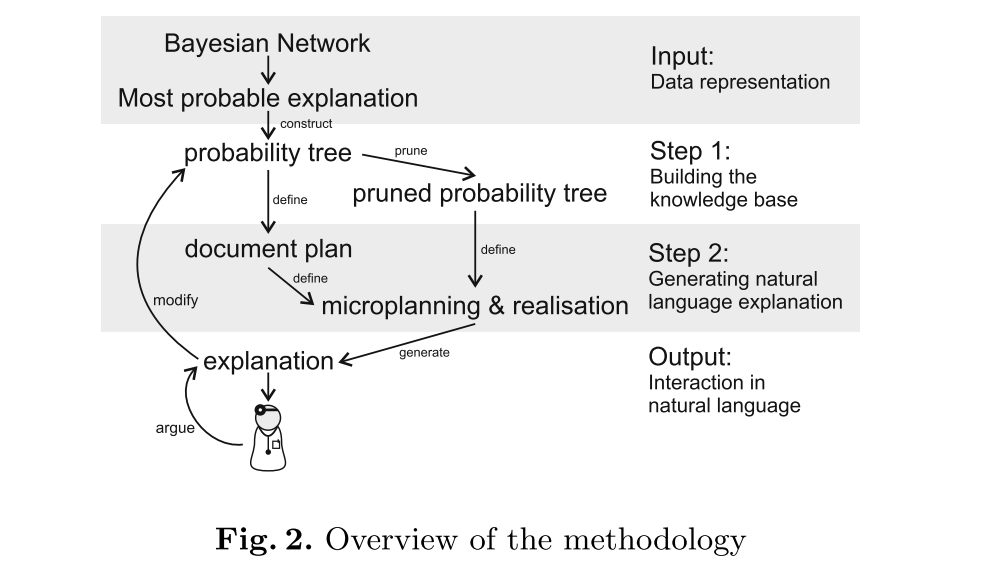
\includegraphics[width=\textwidth]{literature-review/images/butz-methodology}}
\caption{Overview of methodology followed by \citet{Butz2018}}
\label{fig:butz-methodology}
\end{figure}

The document plan for the argumentation follows the same chain of strongest dependencies constructed in the knowledge base until the expert disagrees; at that point, the user is presented with an alternative \enquote{MPE}.
An example of how the document plan may look after interaction with the user is shown in Figure \ref{fig:butz-tree}.
All the natural language phrasing is generated via boilerplates that take care of realising both the micro-planning phase and the generation of the text.

\begin{figure}[htbp]
\centerline{
\includegraphics[width=\textwidth]{literature-review/images/butz-tree}}
\caption{\textit{Document plan} generated from the \textit{probability tree} \citep{Butz2018}}
\label{fig:butz-tree}
\end{figure}

The authors recognise that such chains of deduction could become long and cognitively overloading in the case of larger BNs, as every variable in the tree is explained by all its ancestors.
A solution they propose is that of \textit{pruning} the probability tree by excluding d-separated nodes and those under a certain threshold of significance.
They also adapt some methods from literature to perform \textit{conflict analysis}; that is, only variables that contribute positively to the explanation are maintained in the document plan.

On the whole, \citet{Butz2018} offer a compelling explanation method for BNs by building on an established tradition of explainability through dialogue.
The work, though, takes some methodological missteps and also continues the \enquote{sin} of not validating its claims on real users, one of the primary gaps in the xAI field identified in the previous sections.
\todo{controllare se qualcuno ha lavorato nell'estendere i metodi del paper}

\section{A Progressive Explanation of Inference in \enquote{Hybrid} Bayesian Networks for Supporting Clinical Decision Making}

%%%%
%%%% METHODOLOGY
%%%%

\chapter{Methodology}\label{chap:methodology}
The methodology section of a research paper answers two main questions:

1. How was the data collected or generated?

2. Which methodology was used to analyze it?

In writing the methodology chapter, explain the methodology you are using and why you chose it. Your reader needs to know the method you used to get your data because it effects your findings, and how you interpret your findings. It can be helpful to think of this piece as a ''manual'' - write so that someone can pick up your paper and do the same work you have done. Be direct and precise.

Your methodology is crucial to the quality of your research. It is important that the methodology is appropriate and your reasons for selecting it are clear. You should follow accepted practices; there is no need to re-invent a method. Your literature review can help you determine the method to use.

What  goes  into  Methods  chapter  ?  

It  is  all  about  HOW  you  will  do  the  study   What  is  the  method  ?  

What  does NOT go  into  Methods  chapter  ?  

Results  Implementation

% !TEX root = thesis-thomas-tiotto.tex

\section{Mathematical background}
Bayesian Networks (BN) are a class of Probabilistic Graphical Models that are used to represent systems under conditions of uncertainty.
To give a formal definition we will first need a few basic concepts from probability and graph theory.

\subsection{Probability theory}
\subsubsection{Probability distributions}
\begin{definition}
	A \textit{probability distribution} is a function $\mathbb{P}: \mathcal{S} \rightarrow \mathbb{R}$ with $\mathcal{S}$ a set of \textit{events} of interest.  
To be a valid probability distribution $\mathbb{P}$ must satisfy:
\begin{itemize}
	\item $\mathbb{P}(\sigma) \geq 0 \quad \forall \sigma \in \mathcal{S}$
	\item $\sum_{\sigma} = 1 \quad \forall \sigma \in \mathcal{S}$
	\item $\alpha, \beta \in \mathcal{S} \wedge \alpha \cap \beta=\emptyset 	\Rightarrow \mathbb{P}(\alpha \cup \beta)=\mathbb{P}(\alpha)+\mathbb{P}(\beta)$
\end{itemize}
\end{definition}
Each event $\sigma \in \mathcal{S}$ must have a probability $\mathbb{P}(\sigma) \in [0,1]$ and the sum of all these must equal $1$. 
An event with $P(\sigma) = 0$ is deemed \textit{impossible} while one with $\mathbb{P}(\sigma) = 1$ is \textit{certain}.

There is some discord regarding how to actually \textit{interpret} the probability of an event.
What I believe to be the initially commonly held view is the \textit{frequentist} one, that views the probability of an event as the ratio of times it would occur over a great number of trials.  
So, for example, saying that obtaining a heads has probability $0.5$ when tossing a coin would mean that over repeated throws we would observe heads half the time.

Another, commonly held view is the \textit{Bayesian} (from the 18th century mathematician Thomas Bayes) one in which probabilities are viewed as the \textit{subjective} degree of belief attributable regarding the manifestation of an event.
In this interpretation, stating that a coin has $0.5$ probability of landing on heads simply means that the person making the claim personally believes that the chances of seeing heads of tails are the same.
This is obviously a ``softer'' definition compared to the frequentist one but it is nonetheless useful in that it lets one characterise certain events that haven't come about yet or are liable to happen only once or a few times.

Philosophically, Bayesian inference assigns a probability to a hypothesis (a \textit{prior}) while the frequentist method tests a raw hypothesis empirically before assigning it any probability.
As Bayesian inference naturally embraces and deals with uncertainty, it is an enormously useful tool to model and reason about the real, stochastic world we live in.

\subsubsection{Random variables}
\begin{definition}
	A random variable is a function that associates every outcome in $\mathcal{S}$ with a value.
\end{definition}
\textit{Random variables} are a way of bringing to the fore the attributes of interest of events while dealing with them in a clean, mathematical way.
The values that a random variable can take are a function of the events in sample space $\mathcal{S}$, each of these is assigned a value by the random variable function.
I will only be dealing with \textit{categorical random variables} i.e. those who's codomain is a discrete set of values.
Every random variable has a probability distribution induced by the cardinality of the subsets of its values; in the case of categorical-valued one, such a distribution is \textit{multinomial}.

\subsubsection{Conditional probabilities}
After having defined the basic notion of probability, we can construe one the basic building blocks of Bayesian Networks: the concept of \textit{conditional probability} 
\begin{definition}
	The conditional probability, ``the probability of event $\beta$ given event $\alpha$'' is:
\begin{equation} \label{eq:conditionalprobability}
\mathbb{P}(\beta \mid \alpha) = \frac{\mathbb{P}(\beta \cap \alpha)}{\mathbb{P}(\alpha)}
\end{equation}
\end{definition}
That is, the relative proportion of event $\beta$ compared to event $\alpha$; this intuitively represents the probability of $\beta$ \textit{knowing} that $\alpha$ has already occurred.

Equation \ref{eq:conditionalprobability} can be easily manipulated to obtain another basic element of Bayesian Networks: what is called the \textit{chain rule of conditional probabilities}:
\begin{equation} \label{eq:chainrule}
	\mathbb{P}(\beta \cap \alpha) = \mathbb{P}(\beta \mid \alpha) \mathbb{P}(\alpha)
\end{equation}
This can be generalised to any number of events:
\begin{equation} \label{eq:chainrule}
	\mathbb{P}(\alpha_1 \cap \ldots \cap \alpha_n) = \mathbb{P}(\alpha_n \mid \alpha_1 \cap \ldots \cap \alpha_{n-1}) \ldots \mathbb{P}(\alpha_1 \mid \alpha_2 ) \mathbb{P}(\alpha_1) 
\end{equation}
Intuitively, it means that we can decompose joint probabilities as products of conditional probabilities.  
As we'll see, this is how the values in a Bayesian Network are calculated.

\subsubsection{Independence}
Now, we have just seen in Equation \ref{eq:conditionalprobability} that, in general, $\mathbb{P}(\beta | \alpha) \neq \mathbb{P}(\alpha)$ because $\mathbb{P}(\beta \cap \alpha) \neq \mathbb{P}(\beta) \mathbb{P}(\alpha)$
\begin{definition}
Two events $\alpha$ and $\beta$ are \textit{unconditionally independent} $A \perp B$ - or simply \textit{independent} - when:
\begin{equation}
	\mathbb{P}(\beta \mid \alpha) = \mathbb{P}(\beta) \Leftrightarrow \beta \perp \alpha
\end{equation}
\end{definition}
This means that knowing that $\alpha$ took place doesn't change our beliefs around $\beta$ happening. 
In the real world it is hard, or actually impossible if we consider existence at a fine-enough level to involve Chaos Theory, to find two such perfectly non-interacting events.
Thus, a more useful concept is that of \textit{conditional independence} where two previously dependent event become independent when also conditioned on a third one.
\begin{definition}
Two events $\alpha$ and $\beta$ are \textit{conditionally independent} $(\beta \perp \alpha \mid \gamma)$ when:
	\begin{equation}
	\mathbb{P}(\beta \mid \alpha \cap \gamma ) = \mathbb{P}(\beta \mid \gamma) \Leftrightarrow (\beta \perp \alpha \mid \gamma)
\end{equation}
\end{definition}

\subsection{Graph theory}
Many problems in Machine Learning (ML) don't involve classification or prediction of single data points in isolation, but of set of entities that may present a more, or less, complex relation with each other. 
Most real-world phenomena fit into the latter framework.
Graphs are one of the most powerful tools for the modelling of this class of problems, as their structure naturally captures the wide variety of relations that may exist between entities.
These range from the atomical structure of a molecule to a social network of friends.  
In both these examples graphs help in reasoning, visualising and making inferences and predictions.

\subsubsection{Graphs}
\begin{definition}
	A graph is a tuple 
	\begin{equation}
	\mathcal{G} = (\mathcal{V}, \mathcal{E})
\end{equation}
with $\mathcal{V} = \{ v_1 \ldots v_n \}$ the set of \textit{vertices} and $\mathcal{E} = \mathcal{V} \times \mathcal{V}$ the set of \textit{edges}.
\end{definition}


For our scopes, we will only be considering the case where every element in $\mathcal{E}$ is a pair either of the form $(v_i, v_j)$ or $(v_j, v_i)$ with $i \neq j$.  
That is to say that the class of graphs presently of interest for us are those where there can be at most a single directed edge between any node in $\mathcal{V}$ and no self-loops.
We are also interested in enforcing that there be no \textit{cycles} in the graph, i.e. sequences of nodes of the form $v_i \rightarrow v_j \rightarrow \cdots \rightarrow v_i$.
The resulting graph possessing only directed edges and no cycles is commonly called a \textit{directed acyclic graph}, or DAG for short.  
This data structure is of paramount importance as it's the fundamental graphical representation used for Bayesian Networks.

\subsubsection{Polytrees}
We now have all elements to be able to formally define a Bayesian Network.
I will also define polytrees and trees because these are a fundamental concept for the work carried out in this thesis.
\begin{definition}
	A \textit{loop} is a trace $v_i, v_j \ldots v_i$ of nodes obtained by following edges regardless of their direction
\end{definition}
\begin{definition}
	A directed graph containing no such loops is called a \textit{polytree}. 
\end{definition}
\begin{definition}
	A \textit{tree} is a particular case of polytree where each node has at most one parent.	
\end{definition}

\subsection{Bayesian Networks} \label{subsec:bayesiannetworks}
\begin{definition}
	A Bayesian Network (BN) is a probabilistic graphical model represented by a DAG where each vertex corresponds to a random variable $X_i$ and the edges model the dependencies among these.
\end{definition}
Such a model is basically a way of compactly representing an explicit joint distribution $\mathbb{P}(X_1 \cap \ldots \cap X_n) = \mathbb{P}(X_1) \ldots \mathbb{P}(X_n)$, that is factorised into $\mathbb{P}(X_n \mid X_1 \cap \ldots \cap X_{n-1}) \ldots \mathbb{P}(X_2 \mid X_1 ) \mathbb{P}(X_1) $.
The way this compactness is achieved is in exploiting the independencies that exist among the random variables:
\begin{equation} \label{eq:bnindependencies}
	\forall X_i:  ( X_i \perp \neg Desc(X_i) \mid Pa(X_i))
\end{equation}
with $Pa(X_i)$ the set of nodes that are parents of $X_i$ and $Desc(X_i)$ the nodes that are not \textit{descendents} of $X_i$.
That is to say, every random variable $X_i$, given its parent nodes, is independent of all other nodes in the Bayesian Network that are not descended from it.
Also, a BN gives the flexibility to drop the many weak dependencies that are bound to exist between variables thus leading to an even simpler model.
A full probability table for a joint distribution of random variables obscures the independencies and requires an exponential number of entries for the representation.
A Bayesian Network on the other hand can represent the same distribution using only a linear number of parameters.

One nice characteristic of BNs is that they very naturally model the type of mixed causal and stochastic processes that we find in all of Nature.
Imagine we want to represent the process modelled by joint distribution $\mathbb{P}(B,A) = \mathbb{P}(B) \mathbb{P}(A)$; using the chain rule for conditional probabilities (Eq. \ref{eq:chainrule}) we can write this as $\mathbb{P}(B \mid A) \mathbb{P}(A)$.
A BN modelling this process would be composed of two nodes $A$ and $B$ with an edge from the former to the latter $A \rightarrow B$, $A$ is called the ``parent'' of $B$.  Each of these two nodes would have its own probability table, with $\mathbb{P}(A)$ representing the \textit{prior} distribution over $A$ and $\mathbb{P}(B \mid A)$ the \textit{conditional probability distribution} of $B$ given $A$.

We can now see why these types of models are named \textit{Bayesian} Networks: the inference process is based in a given prior distribution/belief and evolves through a parent $\rightarrow$ child relationship to constantly yield an updated \textit{posterior} belief.
The BN DAG encodes a generative sampling where each variable's value is determined stochastically by Nature, based on the value of its parents.
This process is also highly compatible with our view of causality and this is one of the reason that makes BNs highly interpretable.
The prior $\mathbb{P}(A)$ can be seen as the result of some stochastic process caused by a series of latent (unmodelled) variables while the posterior $\mathbb{P}(B \mid A)$ is stochastically, causally determined by $A$. 
As I have mentioned in the previous paragraphs, there are probably no truly ``prior'' distributions in the Universe, at the modelling scale we are usually interested in.
Only on arriving on the quantum particle level may we find ``pure'' stochastic, uncaused processes due to quantum collapse.

A good example of how BNs are well compatible with our notion of causality may be to imagine $A$ as the random variable modelling the predisposition to having a certain disease and $B$ to actually developing the symptoms for it.
\textit{First}, genetic and epigenetic factors such as the environment stochastically contributed to having the predisposition and \textit{then} the development of the symptoms was stochastically determined by the degree of predisposition.
Adding an extra time dimension certainly helps us in dealing with this class of models.

\subsubsection{d-separation}
The way that Bayesian Networks can be used to reduce the storage requirements for uncertain information is by taking advantage of the conditional independencies embedded in the underlying distribution being modelled.
The power of BNs comes from the additional information encoded in their structure and this was first explicitly described in its entirety by \cite{Pearl1988} who defined the concept of dependence separation, commonly known as \textit{d-separation}.

d-separation, as the name entails, talks about the conditional dependence between variables.
To define it, we first say when two variables $X$ and $Y$ are causally connected.
This is so if $Z = \emptyset$ and they are part of one of the following three structures:
\begin{itemize}
  \item $X \rightarrow Z \rightarrow Y$
  \item $X \leftarrow Z \leftarrow Y$
  \item $X \leftarrow Z \rightarrow Y$
\end{itemize}
This means that knowing something about $X$ also tells us something new about $Y$.
$X$ and $Y$ are causally independent if they appear in the following structure:
\begin{itemize}
  \item $X \rightarrow Z \leftarrow  Y$
\end{itemize}
Such a configuration is called a \textit{collider} and it blocks the flow of information from $X$ to $Y$.
If $Z \neq \emptyset$ the cases are reversed so colliders are open and the other three structures are blocked.
\begin{definition}
	Given disjoint subsets $X, Y, Z \subset \mathcal{X}$, $X$ and $Y$ are d-separated if:
	\begin{itemize}
		\item $Z \neq \emptyset$: no path between $X$ and $Y$ presents a collider
		\item $Z = \emptyset$: there is a collider on every path between $X$ and $Y$
	\end{itemize}
\end{definition}

The independencies between variables are encoded in the structure of the DAG so every distribution whose BN has the same connections between nodes also has the same independencies, regardless of the values of the variables.

\subsection{Bayesian Networks structure learning} \label{subsec:bnstructurelearning}
In many probabilistic models initialisation is fast but then fitting the data is slow (ex. k-means).
For Bayesian Networks the converse is true: fitting is fast as only sums of the counts in the data are needed but identifying the correct graph structure can take super-exponential time.
Learning the Bayesian Network structure from data is commonly known as the Bayesian Network Structure Learning (BNSL) problem.
The methods to solve this problem can be roughly categorised into one of three types.

\subsubsection{Search and Score}
This is the most na{\"i}ve method as it does a brute force search over all the possibile graph structure space - i.e. all DAGs with the same number of variables as the input data - and scores all these depending on some cost function.
This process is super-exponential but though the use of dynamic programming and heuristic search algorithms it can become sub-exponential.
Nonetheless, solving the exact BNSL is only feasible up to $~ 30$ variables.

\subsubsection{Constraint learning}
Methods of this type calculate some measure of correlation to identify the presence and direction of edges between nodes.
A typical test is to iterate over all triplets while testing for conditional independencies.
Thanks to the d-separation properties outlined in Sub-Section. \ref{subsec:bayesiannetworks}, this test is able to identify the correct edges.
The algorithm is quadratic in time in the number of vertices.

\subsubsection{Approximations}
Several heuristical approaches have been developed to be able to find good network structures in an efficient manner.
Examples of these are:
\begin{itemize}
  \item Chow-Liu, that builds a tree approximation of the probability distribution
  \item Greedy hill-climbing, that adds/removes/flips an edge at a time
  \item optimal reinsertion, that iteratively calculates the optimal $Markov blanket$ (the subset of all nodes that are sufficient to determine the value of another subset) of an ever-smaller subset of nodes
\end{itemize}

\subsection{Bayesian Networks updating} \label{subsec:bnupdating}
All the types of inference presented are instances of \textit{diagnostic reasoning}, also known as \textit{abductive reasoning}.  
This type of explanation can either be modelled as a conditional probability or a MAP query and is of fundamental importance in many important problems of machine learning including medical diagnosis, that is of particular interest to us.

\subsubsection{Conditional probability query}
The \textit{updating} problem is the process of updating the probabilities of nodes in the BN based on the observation of the values of other vertices.
This process of conditioning on observed information is also called \textit{data propagation}.

The following algorithm was described by \cite{Normand1992} and applies to our case where the random variables follow a multinomial distribution.
What we want, is to calculate the conditioned probability $\mathbb{P}(B \mid D)$ i.e. the updated probability of node $B$ based on observed evidence $E$.
\begin{definition}
	The conditional probability query for variable $B$ given evidence $E$ is:
\begin{equation} \label{eq:bnupdating}
	\mathbb{P}(B \mid E) = \alpha \pi(B) \lambda(B)
\end{equation}
with $\pi(B) \lambda(B)$ analogous to the \textit{prior} and \textit{likelihood} of $B$, respectively.
\end{definition}
The likelihood of $B$ depends only on the weighted likelihoods of its children $C_1, \ldots ,C_k$:\begin{align}
	\lambda(B) = \prod_l \lambda_{C_l}(B) \\
	\lambda_{C_{l}}(B)=\sum_{C_{l}} \lambda\left(C_{l}\right) P\left(C_{l} \mid B\right)
\end{align}
and its prior similarly depends only on the information received from its parents $A$:
\begin{align}
	\pi(B)=\sum_{A} P(B \mid A) \pi_{B}(A) \\
	\pi_{B}(A)=\alpha \pi(A) \prod_{S_{B}} \lambda_{S_{B}}(A)
\end{align}
The information is propagated down if any variable observed is above $B$ while up if any variable observed lives in the tree rooted in $B$.
Initially all leaf nodes' likelihoods are set at $1$ and the priors of root nodes are assumed to be observable.

\subsubsection{Maximum a posteriori query}
Another common type of question we might ask a BN is the following: ``given evidence $E$ which is the most likely assignment of a subset of variables $Y$?''.
This is know as \textit{Maximum a posteriori (MAP)} inference and is a much harder problem that a conditional probability query.
We are trying to solve the an optimisation problem.
\begin{definition}
As defined by \cite{koller2007introduction}.
Given evidence/observed variables $E=e$, $E \subseteq \mathcal{X}$ and sets $Y \subseteq \mathcal{X} - E$ and $Z = \mathcal{X} - E - Y$, with $\mathcal{X}$ the set of all variables in the BN, the MAP query for $Y$ is the assignment of values $Y=y$ that has maximum probability:
	\begin{equation} \label{eq:map}
	\text{MAP}( Y=y \mid E=e ) = \underset{y}{\text{argmax }}  \sum_z \mathbb{P}(Y=y, Z=z \mid E=e)
\end{equation}
\end{definition}


The MAP problem is hard to solve efficiently; that is it is part of the \textit{NP-hard} complexity class, as proved by \cite{Shimony1994}.
Calculating it in a brute-force way would mean elencating all the possible variable-value tuples and computing their joint probabilities; as these are exponential in the number of variables, the problem is evidently untractable.
Moreover, this is true even in a Bayesian Network.  
Such a model may possess a linear number of parameters but the underlying distribution is still exponential.
Explicitly calculating the MAP defeats the very purpose of the BN, that is computational efficiency.
For this reason, there exist a host of approaches to optimising MAP: elimination algorithms, gradient methods, simulated annealing and other stochastic local searches, belief propagation and integer linear programming.


\subsubsection{Most probable explanation query}
A special case of MAP is the \textit{Most probable explanation (MPE)} that, 
\begin{definition}
	As defined by \cite{koller2007introduction}.
 Given evidence/observed variables $E=e$, $E \subseteq \mathcal{X}$ and $W = \mathcal{X} - E$, the MPE query for $W$ is the assignment of values $W=w$ that has maximum probability:
	\begin{equation} \label{eq:mpe}
	\text{MPE}( W=w \mid E=e ) = \underset{w}{\text{argmax }} \mathbb{P}(W=w \mid E=e)
\end{equation}
\end{definition}

This is an easier problem than MAP, as can be seen by comparing Eq. \ref{eq:map} with Eq. \ref{eq:mpe}; MAP presents both a summation and a maximisation and as such is part conditional probability query, part MPE query.
All algorithms for the computation of MAP obviously apply to MPE too, but there exist efficient algorithms for MPE that do not generalise to MAP.
\todo{quali?}


\subsection{Information theory}
The birth of the field of \textit{information theory} is usually traced back to the seminal paper \enquote{A Mathematical Theory of Communication} (\cite{Shannon1949}) where Claude Shannon set the mathematical basis for the quantification of the amount of \textit{information} transmissible over a noisy channel. 
In his words \enquote{The fundamental problem of communication is that of reproducing at one point, either exactly or approximately, a message selected at another point.}
The concepts of field are broad enough to have influenced practically every other scientific discipline and deep enough to have enabled the \enquote{digital age}, for example by enabling the creation of ever more complicated coding schemes for the compression, reconstruction and obfuscation of digital data.

\subsubsection{Entropy}
In classical mechanical statistics, entropy can be seen as a measure of the uncertainty, or randomness, of a physical system.  
This concept was reapplied by Shannon to measure the amount of randomness in a random variable.
\begin{definition}
	Given a random variable $X$ with probability distribution $\mathbb{P}(X)$, its entropy $\Eta(X)$ is defined as the expected amount of information content carried by $X$ (\cite{Schneider2005}):
\begin{equation} \label{eq:entropy}
	\Eta(X) = \mathbb{E}(I(X)) = \mathbb{E}(-\log (\mathbb{P}(X)) = -\sum_{i=1}^{n} \mathrm{P}\left(x_{i}\right) \log _{b} \mathrm{P}\left(x_{i}\right)
\end{equation}
\end{definition}
The base $b$ of the logarithm defines the unit of measure.  Shannon used $b=2$ as he was dealing with the transmission of digital, binary-coded data; in this case the unit of measure are $bits$.

The simplest example of how information entropy characterises a random variable $X$, is in imagining $X$ to model a coin and the task being to predict the probability of the outcome of a throw being heads.
If the coin is fair, we will not be any more surprised to see the outcome being heads than tails; the entropy is maximum as there is maximum uncertainty regarding the outcome.
However, if the coin is not fair and tails is more probable the we will be more surprised than not to see the outcome being heads.  
The entropy is sub-maximal because there is less uncertainty regarding the outcome: tails is more probable than heads.
If one of the outcomes is impossible, for example if the coin has two heads, then the entropy of the coin is $0$ as there is no uncertainty regarding the result of a toss.

\subsubsection{Normalised entropy/efficiency}
Plain entropy is not a good choice when trying to characterise random variables with different cardinalities of their sample space.
Let us suppose that the objective is to find the variable with the least \enquote{entropic} distribution and we suppose that their values have all been generated by the same process, say Gaussian.
Simply calculating their entropies and ordering them according to this criterion will bias the selection process towards the variables with smallest cardinality.
This is because we supposed them to be distributed in the same way so there will naturally be less uncertainty when there are fewer possible outcomes.
This can easily be understood by imagining the distributions to all be random uniform.

To obviate to this problem we need to \textit{normalise} the entropy so that different-sized variables can be directly compared to each other.
To achieve this, we can look at a measure of normalised entropy or \textit{efficiency}:
\begin{equation} \label{eq:normalisedentropy}
 	\eta(X)=-\sum_{i=1}^{n} \frac{p\left(x_{i}\right) \log _{b}\left(p\left(x_{i}\right)\right)}{\log _{b}(n)}
\end{equation}
From Eq. \ref{eq:normalisedentropy} it can be seen that $\eta(X) \in [0,1]$; it is thus normalised and comparable among distributions.
This ratio expresses the amount of entropy found in the distribution compared to the maximum possible entropy when using $n$ symbols, corresponding to the uniform distribution:
\begin{equation}
\mathrm{H}\left(\underbrace{\frac{1}{n}, \ldots, \frac{1}{n}}_{n}\right) = - \sum_{i=1}^n \frac{1}{n} \log _{b} \left( \frac{1}{n} \right) = -n \cdot \frac{1}{n} \log _{b} \left( \frac{1}{n} \right) = - \log _{b} \left( \frac{1}{n} \right) = \log _{b}(n) 
\end{equation}   

% !TEX root = thesis-thomas-tiotto.tex

\section{Methods}
\subsection{Libraries}
\subsubsection{pomegranate}
Pomegranate (\cite{pomegranate}) is an open-source probabilistic models package for python.
Its core philosophy is that every probabilistic model, from Hidden Markov to Bayesian Network, can be seen as a probability distribution and, as such, can be flexibly composed into hierarchical mixture models (\cite{Schreiber2017}).
The package implements:
\begin{itemize}
	\item Probability Distributions
	\item General Mixture Models
	\item Hidden Markov Models
	\item Bayes Classifiers and Na{\"i}ve Bayes
	\item Markov Chains
	\item \textbf{Bayesian Networks}
	\item Factor Graphs
\end{itemize} 

This package was chosen among others for its good implementation of Bayesian Networks, its clear API and its performance.
The package is written in cython and natively supports multi-core parallelism and out-of-core learning.
Network structure learning from data, described in \ref{subsec:bnstructurelearning}, appears to be particularly efficient, thanks to the implementation of prior knowledge into the graph selection process as described by \cite{schreiber_noble_2017}.
The claim of this novel selection process is that it possesses the speed of a heuristic approach while yielding a far better quality estimate.

pomegranate currently only supports Discrete Bayesian Networks so the random variable of each node must have a categorical distribution.

\textit{Structure learning} from data is achieved using the \texttt{from\_samples} method of the \texttt{BayesianNetwork} class, with the default algorithm being the novel one described by \cite{schreiber_noble_2017}.
The \textit{probability} of a sample is calculated using the \texttt{probability} function of an object of \texttt{BayesianNetwork} type; the \texttt{predict\_proba} function is used to return the probability of each variable in the model given some evidence.
\textit{Predictions} (described in detail in Sec. \ref{subsec:bnupdating}) are run by passing to the \texttt{predict} function of an object a matrix with \texttt{None} as placeholders for missing values .
\textit{Fitting} is done thought the \texttt{fit} function that uses MLE estimates to update each node's distribution in the model based on the input data.

A \texttt{BayesianNetwork} object can also be displayed graphically by calling its \texttt{plot} function.
The output is a DOT file that is generated using the PyGraphviz package (\cite{pygraphviz}), that is a python interface to the famous Graphviz (\cite{graphviz}) graph visualisation software.
An example of such an output is shown in Fig. \ref{fig:pomegranate_graph_example}.

\begin{figure}[htbp]
\centerline{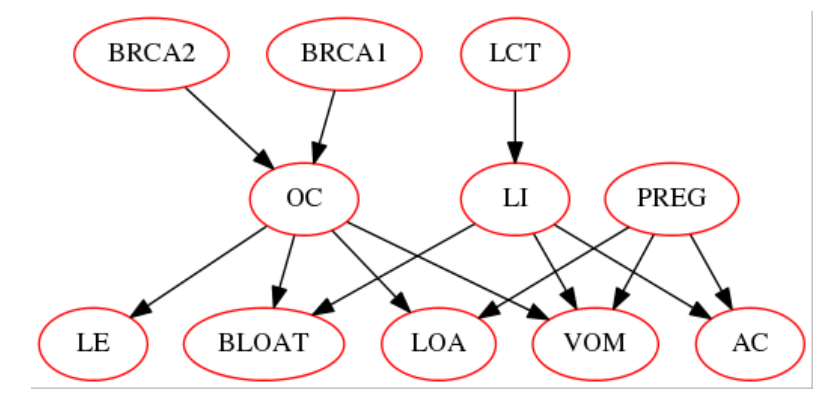
\includegraphics[width=\columnwidth]{methodology/images/pomegranate_example}}
\caption{Example output of \texttt{plot} (\cite{pomegranatetutorial}) }
\label{fig:pomegranate_graph_example}
\end{figure}

\subsubsection{pandas}
\subsubsection{scikit-learn}
\subsubsection{numpy}
\subsubsection{networkx}
\subsection{Algorithms}
\subsubsection{d-separation}
\subsubsection{MPE}
\section{Novel contributions}\label{sec:novel-contributions}
 \todo{tengo qui o sposto nel cap 4?}

\subsection{Theory} \label{subsec:theory}
\todo{la discussione con l'esperto ci da' belief revision dei dati}
\todo{counterfactual explanations}
\todo{magari togliere theory e mettere tutto assieme}

\subsubsection{Selection based on entropy}
\todo{utilizzo entropia}

\subsection{Algorithms}
An important part of my work was developing the algorithms needed to adapt the ideas presented in the paper \enquote{Explaining the Most Probable Explanation} by \cite{Butz2018} and \enquote{A Progressive Explanation of Inference in \enquote{Hybrid} Bayesian} by \cite{Kyrimi2016}.
From the former, the construction of the probability tree through a constructive dialogue with the domain expert, the building of counterfactual explanation branches, the automatic generation of the most probable probability tree from initial evidence.
From the latter, the generation of an \enquote{Inverse explanation}.
Finally, a simple procedure to output a natural language explanation was developed.

\subsubsection{\enquote{Pseudo-MPE}} \label{subsubsec:pseudo-mpe}
\todo{dove critico il fatto che non calcolano veramente l'MPE come dicevano? qui o in cap.4 on cap.2?}
The so-called \enquote{Pseudo-MPE} algorithm is inherently wrapped up with the concept of \textit{dialogue} and is central to the explanatory powers of the system being developed in this thesis.
The algorithm was developed as a way of implementing the \enquote{MPE branch} of the \enquote{Argumentative Probability Tree} hypothesised by \cite{Butz2018}.
It was termed \enquote{Pseudo-MPE} because there are no guarantees of it returning the MPE solution (see Subsec. \ref{subsec:bnupdating}), as noted by \cite{koller2007introduction} in their definition of the MAP problem.

At a lower level of detail, the algorithm may be broken into:
\begin{itemize}
	\item a dialogical part, that interfaces with the expert user through the use of natural language, menus and visualisations
	\item the part responsible for constructing the \enquote{MPE branch}
\end{itemize}
The former process was informed and shaped by the results obtained by the methods described in Subsec. \ref{subsec:explainability-validation} and, as such, presented substantial elements of novelty.

The latter process is, at its core, a greedy procedure that aims at selecting the \enquote{best} next $(state, value)$ tuple at each step, based on some measure of optimality and on the variables already in the evidence set.
In the actual implemented system the two parts are intertwined, given their close inter-dependence.

The \texttt{dialogue} procedure starts by asking the user to select a subset of variables and their relative values to add as initial evidence.
This initial evidence is used to radicate the MPE Branch.
It should be noted than in the description given by \cite{Butz2018}, the Argumentative Probability Tree is a real tree as each node is guaranteed to have at most one parent.
My application, on the other hand, constructs an \textit{Argumentative Probability Polytree} (see Subsec. \ref{subsec:polytrees}) because, as will better be described in Chap. \ref{chap:results}, it was seen early on that the users much preferred to be able to start from a set of initial evidences and not be limited to a single one.
The algorithm then proceeds to call the \texttt{next\_most\_probable\_states} subroutine that is tasked with returning an ordered list of $(state,value)$ pairs.
It does this by calculating the posterior distribution given evidence of all the states not already in the evidence, then calculating the efficiency (see \ref{subsec:normalised-entropy}) and the maximally probable symbol of each state's distribution and finally returning the $(state,value)$ tuples ordered according to their normalised entropy (most efficient/least entropic at the head).
The $(state,value)$ pair at the head of the list is proposed to the user who has the faculty to accept the system's evaluation or refuse it.
If the user accepts, the state is added to the evidence set and to the MPE Branch under construction.
Thus, the evidence set's cardinality increases by one each time a user accepts a proposal.
The updated evidence will be used to calculate the new list of $(state,value)$ pairs at the following round.
If the expert chooses to refuse, then she is iteratively presented with the remaining $(state,value)$ items, in order of decreasing efficiency. 
Once she accepts one of the explanations given by the system, the \texttt{generate\_alternative\_branch} subroutine is called to automatically generate a maximally probable MPE Branch, radicated in the newest $(state,value)$ node of the MPE Branch.
The proposal loop for alternative states runs until there are increasingly less probable elements in the list and exits with a partial solution if the user refuses all of them at a given step.
Thus, the Pseudo-MPE solution is constructed only if the user runs through all variables proposed, accepting each one at least once.

Three slightly different operational modes of the algorithm were implemented.
This was done for research purposes, in order to understand which of the three, if any or if a combination of their distinctive features, the expert users would find the most useful from a usability, comprensibility and explainability standpoint:
\begin{itemize}
  \item exhaustive: In the basic dialogue type, the set of variables under consideration monotonically decreases by one every time the user accepts one of the system's proposals and the dialogue terminates only when the user has accepted all variables at least once or refused all proposals at a given step.
	In the first case the user will have the Pseudo-MPE solution while in the second she will be left with a partial assignment to some of the variables not present in the initial evidence.
	The pseudocode is shown in Alg. \ref{alg:pseudo-mpe-exhaustive}.
  \item d-separated: In the second variant, the set of variables under considered at each step is dynamic and depends on the separation properties of the underlying Bayesian Network's DAG and the evidence set constructed by the user's choices.
  	Differently from the first type of dialogue, an additional \texttt{evidence\_d\_separation} subroutine is called before \texttt{next\_most\_probable\_states} to calculate the set of variables that are d-separated from the evidence set, up to that step of the dialogue.
  	\texttt{next\_most\_probable\_states} is then executed but the variables that the previous function found to be separated from the evidence, are removed from the returned list.
  	This way, variables that can have no effect given the current evidence are not proposed.
  	As the d-separation operation is not monotonic, adding new nodes to the evidence set can both increment or diminish the number of nodes that will be proposed at each step.
  	The user is shown an updated view of the independencies of the graph at each step; an example of such an output is shown in Fig. \ref{fig:pseudo-mpe-independencies_1} and \ref{fig:pseudo-mpe-independencies_2}.
  	The pseudocode is shown in Alg. \ref{alg:pseudo-mpe-independencies}.
  \item thresholded: The final variant of the algorithm prunes the set of variables using a different strategy from the previously presented one.
  	In this case, the $(state,value)$ pairs in the list returned by \texttt{next\_most\_probable\_states} are dropped automatically based on their probability.
  	Pairs whose probability is below a user-defined threshold or are \enquote{worse than random} (for ex. a $(state,value)$ tuple will be discarded if $state$ is binary and the probability of $value$ is lower than $0.5$) are removed and not proposed to the user. 
  	This thresholding strategy based on the probability of the tuples is paired with one where there is a user-defined threshold on the number of times that the expert can refuse a particular $(state,value)$. 
  	In the general dialogue, tuples can be proposed multiple times, with an ever lower probability, if the user has previously refused them; in the thresholded scheme a $(state,value)$ pair can only be proposed a maximum number of times before being permanently discarded.
\end{itemize}

The underlying Bayesian Network that represents the data set is learned and queried through the  \texttt{pomegranate} (see Subsec. \ref{subsec:libraries}), API but the great majority of all the code is completely custom-written.
This was necessary because \texttt{pomegranate}, while having a powerful backend, was found to be severely lacking in the breadth and flexibility of its API.
Many basic operations, such as the calculation of a joint distribution, were not available so the only way was to implement lower-level workarounds while still using \texttt{pomegranate} for the most basic operations, as the calculation of a posterior distribution.
In particular, \texttt{dialogue} is implemented with the only direct calls to the API being when learning the network and when calling \texttt{predict\_proba}, that queries the \texttt{BayesianNetwork} object to calculate the posterior distribution of the states given the current evidence.
D-separation, in the second variant of the algorithm, is calculated via the \texttt{evidence\_d\_separation} procedure that implements the pseudocode presented in Alg. \ref{alg:d-separation}.

\begin{algorithm}[htp!]
	\caption{Exhaustive pseudo-MPE algorithm}
	\label{alg:pseudo-mpe-exhaustive}
	\begin{algorithmic}[1]
		\State $evidence = $ user selected $(state,value)$ tuples
		\State $MPE\_polytree = $ MPE Polytree rooted in $evidence$
		\While{True} 
			\State $mpe\_states$ = \texttt{next\_most\_probable\_states($evidence$)}
			\If{$mpe\_states$ is not empty}
				\State $next\_state$ = head of $mpe\_states$ 
				\State propose $next\_state$ to user \Comment{the least entropic state}
				\If{the user refuses $next\_state$}
					\For{$alternative\_state$ in $mpe\_states \smallsetminus next\_state$}
						\State propose $alternative\_state$ to user \Comment{the next least entropic states}
						\If{the user accepts $alternative\_state$}
							\State call \texttt{generate\_alternative\_branch()} on $MPE\_polytree$ 
							\State add $alternative\_state$ to $MPE\_polytree$
							\State $evidence = evidence \cup alternative\_state$
						\Else
							\State continue
						\EndIf
					\EndFor
				\Else
					\State add $next\_state$ to $MPE\_polytree$
					\State $evidence = evidence \cup next\_state$
				\EndIf
			\Else 
				\State return
			\EndIf
		\EndWhile
	\end{algorithmic}
\end{algorithm} 

\begin{algorithm}[htp!]
	\caption{Independencies pseudo-MPE algorithm}
	\label{alg:pseudo-mpe-independencies}
	\begin{algorithmic}[1]
		\State $evidence = $ user selected $(state,value)$ tuples
		\State $MPE\_polytree = $ MPE Polytree rooted in $evidence$
		\While{True} 
			\State $separated = $ \texttt{evidence\_d\_separation($evidence$)} \Comment{based on evidence of previous step}
			\State $mpe\_states$ = \texttt{next\_most\_probable\_states($evidence$)}
			\State $mpe\_states = mpe\_states \smallsetminus separated$ 
			\If{$mpe\_states$ is not empty}
				\State $next\_state$ = head of $mpe\_states$ 
				\State propose $next\_state$ to user \Comment{the least entropic state}
				\If{the user refuses $next\_state$}
					\For{$alternative\_state$ in $mpe\_states \smallsetminus next\_state$}
						\State propose $alternative\_state$ to user \Comment{the next least entropic states}
						\If{the user accepts $alternative\_state$}
							\State call \texttt{generate\_alternative\_branch()} on $MPE\_polytree$ 
							\State add $alternative\_state$ to $MPE\_polytree$
							\State $evidence = evidence \cup alternative\_state$
						\Else
							\State continue \Comment{go to next proposal}
						\EndIf
					\EndFor
				\Else
					\State add $next\_state$ to $MPE\_polytree$
					\State $evidence = evidence \cup next\_state$
				\EndIf
			\Else 
				\State return 
			\EndIf
		\EndWhile
	\end{algorithmic}
\end{algorithm} 

\begin{figure}[htbp]
\centerline{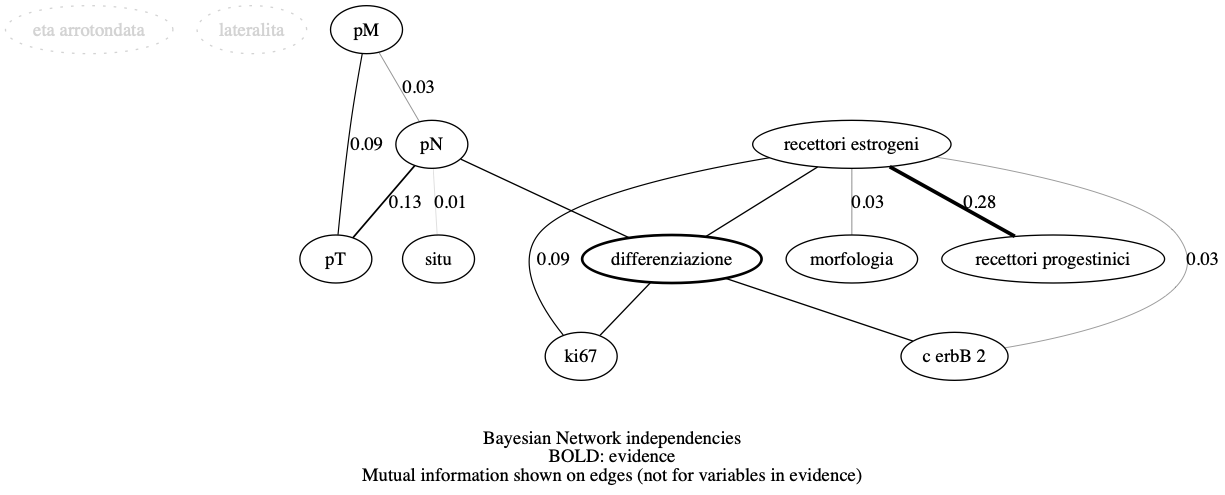
\includegraphics[width=\columnwidth]{methodology/images/example-d-separation-mpe_1}}
\caption{Example output during the first round of the d-separation-aware variant of \texttt{dialogue}.
	The variable \enquote{mut17q21} is the initial evidence.}
\label{fig:pseudo-mpe-independencies_1}
\end{figure}

\begin{figure}[htbp]
\centerline{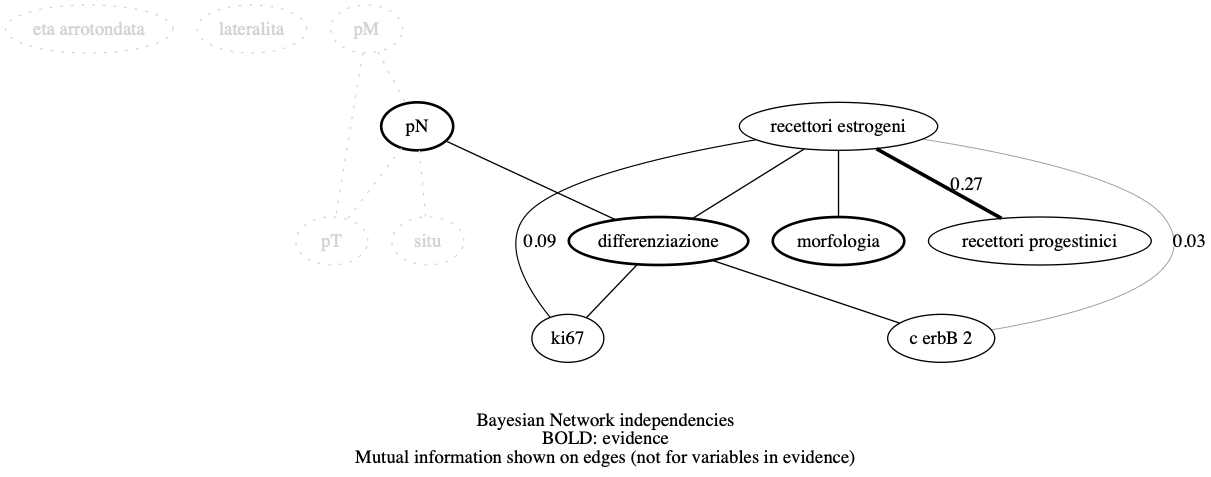
\includegraphics[width=\columnwidth]{methodology/images/example-d-separation-mpe_2}}
\caption{Example output during the second round of the d-separation-aware variant of \texttt{dialogue}.
	\enquote{morfologia} is added to the evidence set and this makes a large part of the network redundant.}
\label{fig:pseudo-mpe-independencies_2}
\end{figure}

\begin{algorithm}[htp!]
	\caption{Thresholded pseudo-MPE algorithm}
	\label{alg:pseudo-mpe-thresholded}
	\begin{algorithmic}[1]
		\State user selected $refuse\_bound$
		\State $refuse\_thresholds = \emptyset$
		\State $lower\_thresholds = \emptyset$
		\For{$v \in V$}
			\For{value $k$ of $v$}
				\State element $[v,k]=0$ in $refuse\_thresholds$
			\EndFor
			\State element $[v]=1 / |v|$ in $lower\_thresholds$ \Comment{refuse worse than random pairs}
		\EndFor
		\State $evidence = $ user selected $(state,value)$ tuples
		\State $MPE\_polytree = $ MPE Polytree rooted in $evidence$
		\State $mpe\_states$ = \texttt{next\_most\_probable\_states($evidence$)}
		\While{True} 
			\For{$s \in mpe\_states$}
				\If{probability of $s < lower\_thresholds[s] \wedge refuse\_thresholds[s] > refuse\_bound$}
					\State remove $s$ from $mpe\_states$ 
				\EndIf
			\EndFor		
			\If{$mpe\_states$ is not empty}
				\State $next\_state$ = head of $mpe\_states$ 
				\State propose $next\_state$ to user \Comment{the least entropic state}
				\If{the user refuses $next\_state$}
					\State increment $refuse\_thresholds[next\_state]$
					\For{$alternative\_state$ in $mpe\_states \smallsetminus next\_state$}
						\State propose $alternative\_state$ to user \Comment{the next least entropic states}
						\If{the user accepts $alternative\_state$}
							\State call \texttt{generate\_alternative\_branch()} on $MPE\_polytree$ 
							\State add $alternative\_state$ to $MPE\_polytree$
							\State $evidence = evidence \cup alternative\_state$
						\Else
							\State increment $refuse\_thresholds[alternative\_state]$
							\State continue
						\EndIf
					\EndFor
				\Else
					\State add $next\_state$ to $MPE\_polytree$
					\State $evidence = evidence \cup next\_state$
				\EndIf
			\Else 
				\State return
			\EndIf
		\EndWhile
	\end{algorithmic}
\end{algorithm} 

\subsubsection{Alternative Explanation Branches}
The function to generate alternative branches to the main MPE branch in the dialogue tree is called after the user refuses a $(state,value)$ in the dialogue and accepts one of the the alternatives.
The motivation is to present the user with a simple \enquote{what-if} analysis, replying to the question \enquote{Had I accepted the $(state,value)$ presented me by the system, what would have been the most probable configuration of the remaining $(state,value)$ pairs?}.
The question is answered by generating a maximally probable, alternative MPE sub-branch rooted in the last node in the main MPE branch that is under construction through the dialogue.

The alternative branch is generated by what is essentially an automated version of \texttt{dialogue} that always accepts the first suggestion returned by \texttt{next\_most\_probable\_states}.
Given that \texttt{dialogue} and \texttt{generate\_alternative\_branch} are essentially one and the same, the latter inherits the same pruning strategies as the former.
That is, \texttt{generate\_alternative\_branch} called during the exhaustive dialogue will generate a maximally likely assignment over all variables in $V \smallsetminus E$ while when invoked from one of the other two variant of the dialogue algorithm, it will apply their same pruning strategies.

The implementation of the MPE Polytree is based on the \texttt{NetworkX} python package (see Subsec. \ref{subsec:libraries}).
The creation of a chain of nodes is done by keeping a local pointer $alt\_node$ that refers to the last added node or set of nodes, if the node being added is the successor of multiple initial evidences. 

An example of the output shown to the user at each step of the dialogue is shown in Fig. \ref{fig:alternative-branch} while the pseudocode for the three variants are shown in Alg. \ref{alg:alternative-branch-echaustive}, \ref{alg:alternative-branch-independencies} and \ref{alg:alternative-branch-thresholded}.
Note that $alternative\_evidence$ is local to this algorithm and is separate from the $evidence$ used in the main \texttt{dialogue} procedure.

\begin{figure}[htbp]
\centerline{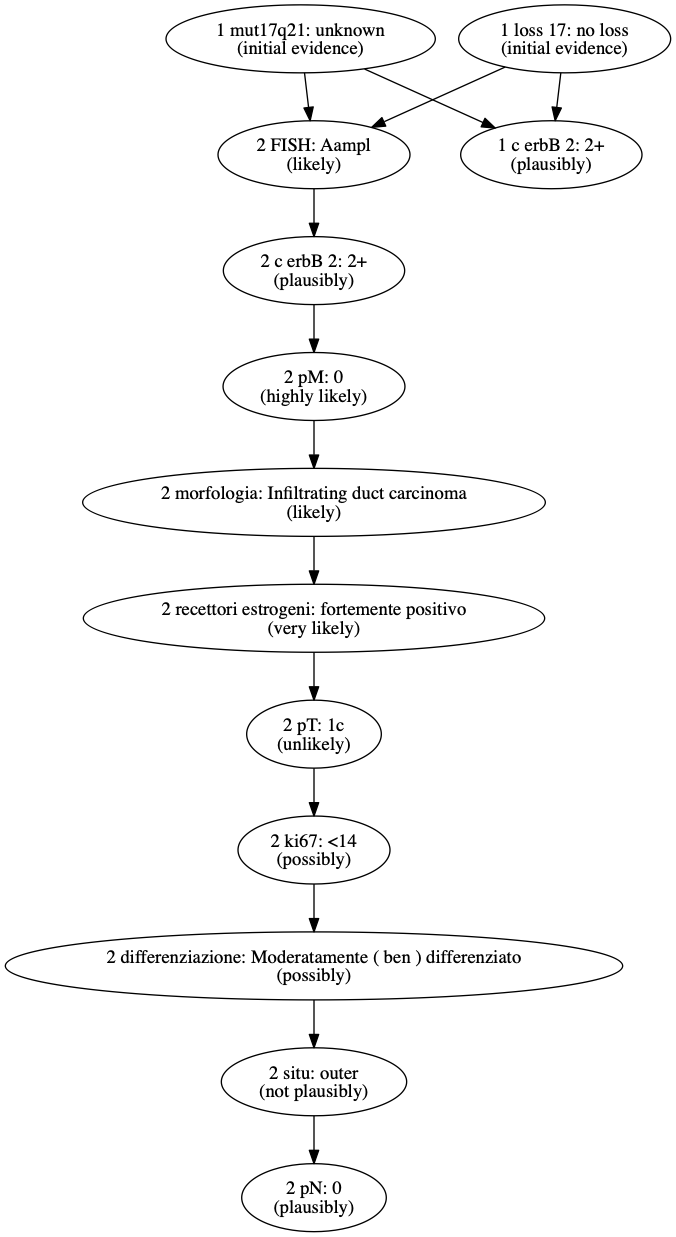
\includegraphics[scale=0.2]{methodology/images/alternative-explanation-tree-example}}
\caption{Example output during the d-separation-aware variant of \texttt{dialogue}.
	The tuple (\enquote{FISH},\enquote{Aampl}) was proposed but the expert refused it and accepted the alternative (\enquote{c erbB 2},\enquote{2+}).
	The main MPE Branch has ID 1 while the \enquote{what-if} one has ID 2.}
\label{fig:alternative-branch}
\end{figure}

\begin{algorithm}[htp!]
	\caption{Exhaustive alternative explanation branch algorithm}
	\label{alg:alternative-branch-echaustive}
	\begin{algorithmic}[1]
		\State $alternative\_evidence = evidence$ 
		\State $alt\_node = $ last node in the main MPE Polytree
		\State $branch\_id = branch\_id + 1$
		\While{True} 
			\State $mpe\_states$ = \texttt{next\_most\_probable\_states($alternative\_evidence$)}
			\If{$mpe\_states$ is empty}
				\State return
			\Else
				\State $next\_state$ = head of $mpe\_states$ 
				\State create $next\_state$ node, tag it with $branch\_id$ and make it son of $alt\_node$
				\State update $alt\_node$ node to be $next\_state$ node
				\State $alternative\_evidence = alternative\_evidence \cup next\_state$
			\EndIf
		\EndWhile
	\end{algorithmic}
\end{algorithm}

\begin{algorithm}[htp!]
	\caption{Independencies alternative explanation branch algorithm}
	\label{alg:alternative-branch-independencies}
	\begin{algorithmic}[1]
		\State $alternative\_evidence = evidence$ 
		\State $alt\_node = $ last node in the main MPE Polytree
		\State $branch\_id = branch\_id + 1$
		\While{True} 
			\State $separated = $ \texttt{evidence\_d\_separation($alternative\_evidence$)}
			\State $mpe\_states$ = \texttt{next\_most\_probable\_states($alternative\_evidence$)}
			\State $mpe\_states = mpe\_states \smallsetminus separated$ 
			\If{$mpe\_states$ is empty}
				\State return
			\Else
				\State $next\_state$ = head of $mpe\_states$ 
				\State create $next\_state$ node, tag it with $branch\_id$ and make it son of $alt\_node$
				\State update $alt\_node$ node to be $next\_state$ node
				\State $alternative\_evidence = alternative\_evidence \cup next\_state$
			\EndIf
		\EndWhile
	\end{algorithmic}
\end{algorithm} 

\begin{algorithm}[htp!]
	\caption{Thresholded alternative explanation branch algorithm}
	\label{alg:alternative-branch-thresholded}
	\begin{algorithmic}[1]
		\State $alternative\_evidence = evidence$ 
		\State $alt\_node = $ last node in the main MPE Polytree
		\State $branch\_id = branch\_id + 1$
		\While{True} 
			\For{$s \in mpe\_states$}
				\If{probability of $s < lower\_thresholds[s] \wedge refuse\_thresholds[s] > refuse\_bound$}
					\State remove $s$ from $mpe\_states$ 
				\EndIf
			\EndFor	
			\State $mpe\_states$ = \texttt{next\_most\_probable\_states($alternative\_evidence$)}
			\If{$mpe\_states$ is empty}
				\State return
			\Else
				\State $next\_state$ = head of $mpe\_states$ 
				\State create $next\_state$ node, tag it with $branch\_id$ and make it son of $alt\_node$
				\State update $alt\_node$ node to be $next\_state$ node
				\State $alternative\_evidence = alternative\_evidence \cup next\_state$
			\EndIf
		\EndWhile
	\end{algorithmic}
\end{algorithm} 

\todo{ancora da implementare true MPE}
\subsubsection{\enquote{Pseudo-MPE} from Random Evidence} \label{subsubsec: pseudo-mpe-random}
In order to compare the Pseudo-MPE output with the true MPE solution I implemented a simple algorithm that, starting from a random initial set of evidence, generates the relative pseudo-MPE and MPE solutions.
The random initial evidence set is constructed by randomly choosing a number in the interval $k = [ 1, |V| ]$, with $V$ the set of vertices in the BN, and then randomly selecting $k$ of the random variables in $V$ to yield the set of variables $E$.
The value of each variable is randomly chosen among the set of its values; as all variables are categorical, this can easily be done.

The implementation is based on the \texttt{NetworkX} python library (see Subsec. \ref{subsec:libraries}) package as what is being constructed is not a tree but a \textit{polytree} (see Subsec. \ref{subsec:polytrees}), as nodes may have multiple parents.
Note that $alternative\_evidence$ is considered separate from the main $evidence$ used in \texttt{dialogue}.

The pseudocode is shown in Alg. \ref{alg:pseudo-mpe-random-evidence} while an example output can be seen in Fig. \ref{fig:pseudo-mpe-random}.

\begin{algorithm}[htp!]
	\caption{Pseudo-MPE from random evidence algorithm}
	\label{alg:pseudo-mpe-random-evidence}
	\begin{algorithmic}[1]
		\State $evidence = \emptyset$
		\State generate random number $k \in [ 1, |V| ]$
		\State $S = $ choose $k$ variables from $V$
		\For{$s \in S$}
			\State choose random $v$ in the possible values of $e$ 
			\State $evidence = evidence \cup (s,v)$
		\EndFor
		\State $MPE\_polytree = $ MPE Polytree rooted in $evidence$
		\State $last\_node = evidence$
		\State $alternative\_evidence = evidence$ 
		\While{True} 
			\State $mpe\_states$ = \texttt{next\_most\_probable\_states($alternative\_evidence$)}
			\If{$mpe\_states$ is empty}
				\State return
			\Else
				\State $next\_state$ = head of $mpe\_states$ 
				\State create $next\_state$ node and make it son of $last\_node$
				\State update $alt\_node$ node to be $next\_state$ node
				\State $alternative\_evidence = alternative\_evidence \cup next\_state$
			\EndIf
		\EndWhile
	\end{algorithmic}
\end{algorithm}

\begin{figure}[htbp]
\centerline{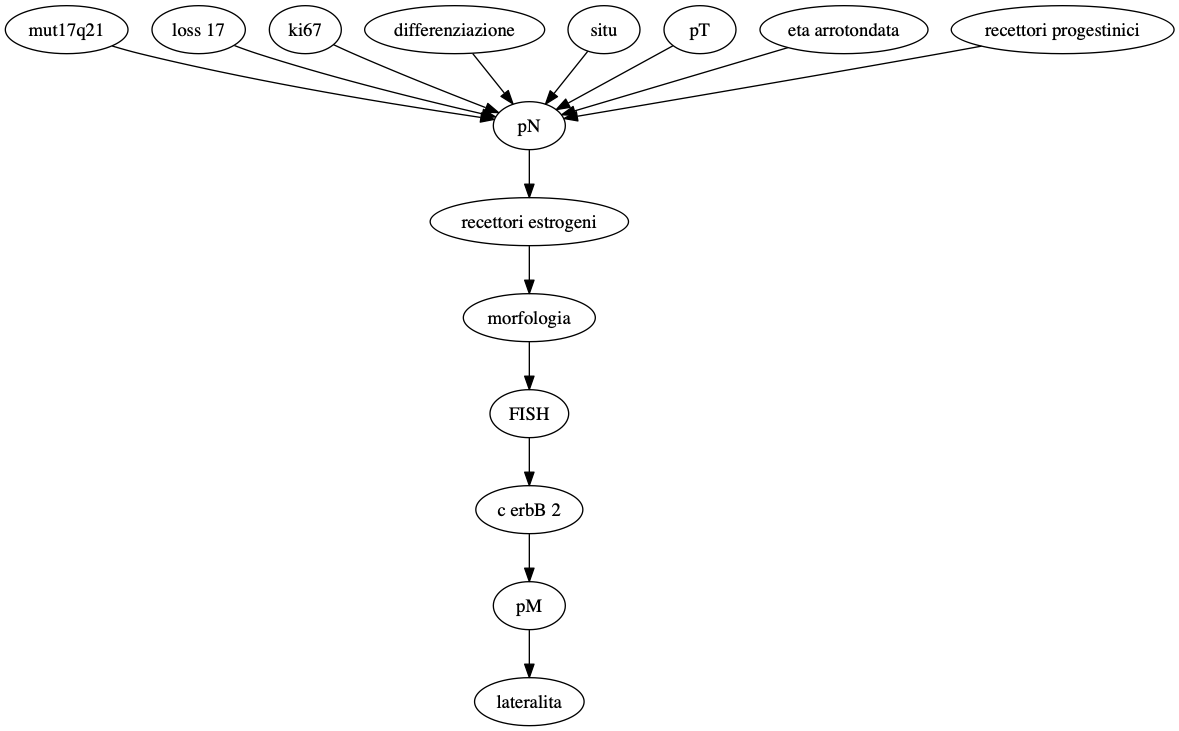
\includegraphics[width=\columnwidth]{methodology/images/pseudo-mpe-random-example}}
\caption{Example output of the Pseudo-MPE from random evidence algorithm.}
\label{fig:pseudo-mpe-random}
\end{figure}

\subsubsection{Inverse Explanation}
\todo{da fare e trovare nome migliore}

\subsubsection{Natural Language Explanation}
\todo{da fare e magari pensare anche a visual explanations?}
The probability of each proposed tuple is quantified in natural language based on the probability of the most probable value within the variable.
These are shown in Tab. \ref{tab:naturallanguageprobabilities}.

\begin{table*}[htbp]
\caption{Probability quantifiers in natural language}
\begin{tabularx}{\textwidth}{@{} X X @{}}
\toprule 
Probability range & Natural language quantifier \\
\midrule 
(0, 0.2) &  "highly unlikely" \\
(0.2, 0.3) & "very unlikely" \\
(0.3, 0.4) & "unlikely" \\
(0.4, 0.5) & "not plausibly" \\
(0.5, 0.6) & "plausibly" \\
(0.6, 0.7) & "possibly" \\
(0.7, 0.8) & "likely" \\
(0.8, 0.9) & "very likely" \\
(0.9, 1) &  "highly likely" \\
(1) &  "certain" \\
\bottomrule
\end{tabularx}
\label{tab:naturallanguageprobabilities}
\end{table*}


\subsubsection{Pairwise Correlations}
An interesting addition, in terms of both explainability and theory, is an algorithm to measure and graphically display the interrelatedness between pairs of variables.
This is achieved by calculating the \textit{conditional mutual information} \todo{AA: e' giusto così?} between each pair of parent $\rightarrow$ child variables.
The definition of mutual information presented in Subsec. \ref{subsec:mutualinformation} is extended to account for the current state of the model i.e. the set of observed variables.
What we are calculating is:
\begin{equation}
	I(X,Y|E=e) = \sum_{x \in \mathcal{X}} \sum_{y \in \mathcal{Y}} p_{XY}(x,y|E=e) \log \left( \frac{p_{XY}(x, y|E=e)}{p_{X}(x|E=e) p_{Y}(y|E=e)} \right)
\end{equation}
This is not done if the parent variable, in the $X \rightarrow Y$ tuple under consideration, is in the evidence set; this is because observing a variable in a BN conceptually corresponds to disconnecting it from its children.

The implementation takes advantage of pgmpy's (\cite{pgmpy}) inference capabilities. 
To do this, I wrote a function to convert a pomegranate-based BN to an equivalent pgmpy-based one.
The queries to the model are done using the variable Elimination algorithm, that is more than suitable for a small BN.
The marginals for $X$ and $Y$ are calculated directly from the joint distributions, by marginalising the joint over one and then the other.
The function exits with $-1$ if the parent variable is in the evidence set.
As the mutual information $I(X,Y) \in [0,1]$ this signals to the calling function to treat this couple $X,Y$ differently.

The pseudocode for the algorithm is shown in Alg. \ref{alg:mutual-information}.

\begin{algorithm}[htp!]
	\caption{Mutual information algorithm}
	\label{alg:mutual-information}
	\begin{algorithmic}[1]
		\State $X$ parent variable in the BN DAG
		\State $Y$ child variable in the BN DAG
		\State $E$ set of current evidence in the BN
		\If{$X \in E$}
			\State return -1
		\EndIf
		\State $joint=p_{XY}(X, Y|E=e)$
		\State $Y\_marginal=$ marginalise $joint$ over $X$
		\State $X\_marginal=$ marginalise $joint$ over $Y$
		\State $mutual\_information = 0$
		\For{y in $Y\_marginal$}
			\For{x in $X\_marginal$}
				\State $j=$entry in $joint$ corresponding to $y$ and $x$
				\If{$j$ is $0$}
					\State $mutual\_information += 0$
				\Else
					\State $mutual\_information = j * log( j / ( y * x ) )$
				\EndIf
			\EndFor
		\EndFor
		\State return $mutual\_information$
	\end{algorithmic}
\end{algorithm}
\section{The Benchmark Data Set} \label{sec:data-set}
This section focuses on presenting the data set that was the basis for the methods developed in this chapter.
The data set was provided by the Istituto Cantonale di Patologia and preprocessed in order to be used to learn a Bayesian Network.

\subsection{The Medical Partner: Istituto Cantonale di Patologia} \label{subsec:istituto-cantonale}
Istituto Cantonale di Patologia (ICP)\footnote{\url{https://www4.ti.ch/dss/dsp/icp/istituto/}} is an institute based in Locarno that is specialised in the histological analysis of tissue samples received from private patients, clinics and hospitals, mainly in support of cancer diagnosis.
Its Laboratory of Molecular Pathology supports the diagnostic approach to neoplastic diseases through the application of biomolecular and cytogenetics techniques, which focus on understanding the impact of molecular alterations in carcinogenesis.
One of the methods used is Fluorescence in Situ Hybridization (FISH) (see Figure \ref{fig:fish-picture} for an example of the results of this technique) that is able to localise the presence or absence of specific DNA sequences in chromosomes.
These tests are aimed at identifying the precise profile of the cancer cells and thus inform the clinician on the best treatment for the specific patient.

\begin{figure}[htbp]
\centerline{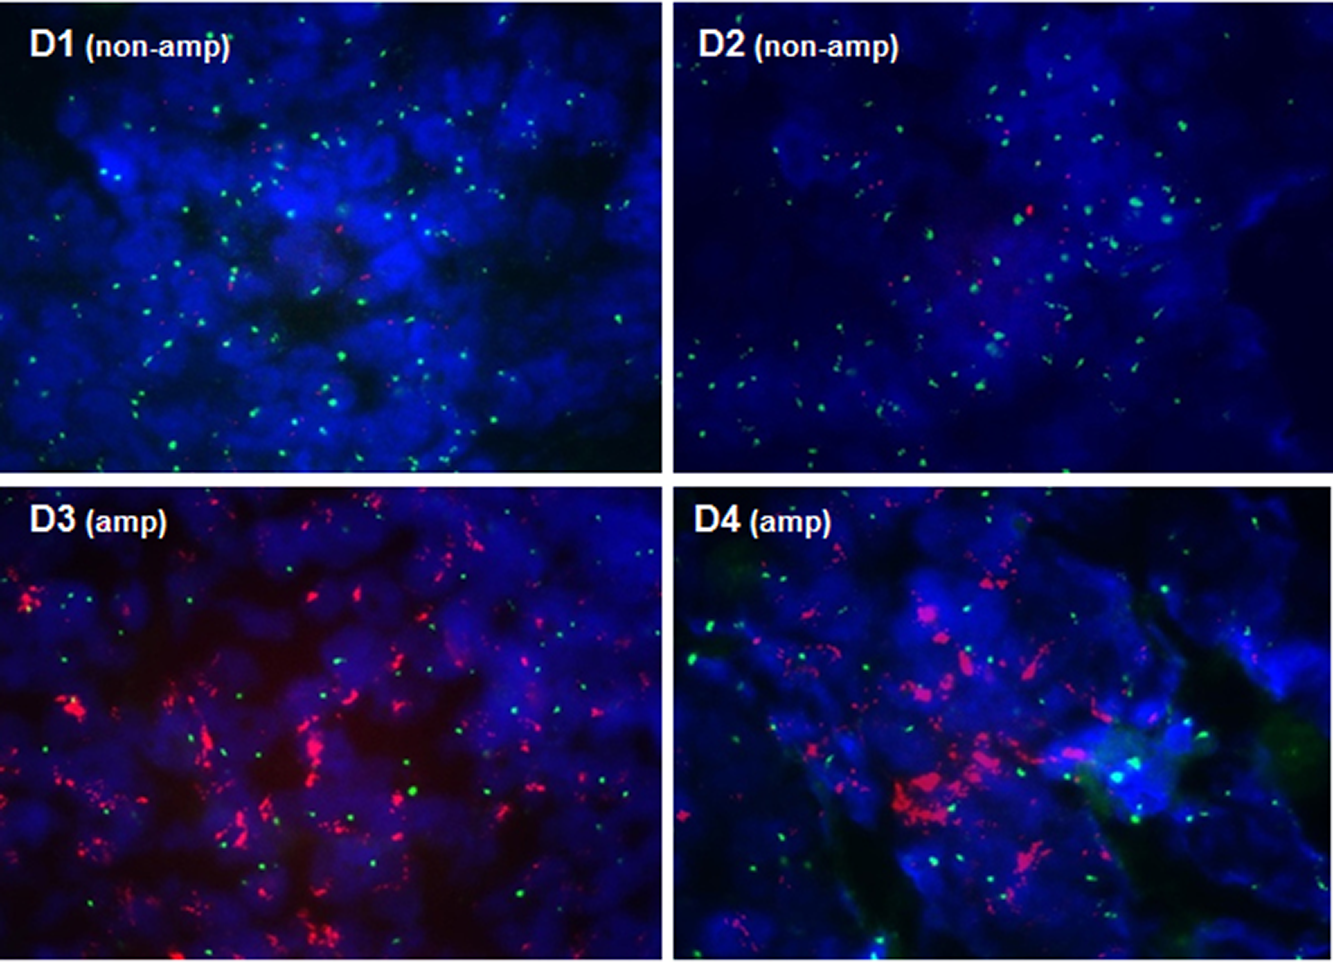
\includegraphics[width=0.8\textwidth]{methodology/images/fish-picture}}
\caption{FISH analysis of HER2 gene expression in samples of breast tumour. The probe mix consists of a mixture of Texas Red-labelled DNA probe against HER2 gene (which is located on chromosome 17) and a fluorescein (green)-labelled probe targeted at the centromeric region of chromosome 17. The upper panels (D1 and D2) show normal expression - 2 green and 2 red signals per cell. The lower panels (D3 and D4) show HER2 amplification whereby there is a clear increase in the red signal. [source: https://www.bioivt.com/fluorescent-in-situ-hybridization-fish/]}
\label{fig:fish-picture}
\end{figure}

Molecular diagnosis is the most recent approach in pathology. It mainly aims to support pathologists in the diagnosis of neoplastic diseases through the employment of molecular biology and cytogenetics techniques and it enables the deep understanding and monitoring of patients' profiles, as well as as defining the prognosis and ad-hoc therapies. All together, it allows the development of an increasingly personalised medicine, also in terms of research (e.g. understanding of pathological mechanisms and thus the possibilities of intervention).
However, it is still limited in its capabilities by the presence of a dishomogeneous information pool, especially in terms of knowledge extraction; a non-uniform data set entails, for the pathologist, an increased cognitive complexity because of having to manage a high number of variables and heterogeneous meaning behind the data; these consequently force to resort to problem decomposition and reduction.

In addition to its clinical support activities, the ICP also carries out scientific research aimed at better understanding certain types of cancers at translational level i.e., at the level of protein synthesis.
In the last ten years, the ICP has published more than 200 peer-reviewed papers and more than 100 works in non-peer reviewed journals and is active at a national and international level.

\subsection{Motivation} \label{subsec:motivation}
The Istituto Cantonale di Patologia already had a collaboration in place with the Dalle Molle Institute for Artificial Intelligence (IDSIA)\footnote{\url{http://www.idsia.ch}} to investigate a series of specific issues, whose details are outside of the scope of this thesis.
The prospect of the work to be carried out in this thesis was deemed of interest because it extended beyond the existing collaboration.
The institute had originally expressed interest in bringing machine learning into their workflow in order to both augment its profiling capabilities for patients and to be able to extract new knowledge from their existing data; this was paired with an attention for more experimental research directions, as the facilitation of human-machine interaction.

Given that the theoretical work carried out in this thesis is, at its core, an investigation into the explainability of Bayesian Networks, collaboration with the Institute provided the precious opportunity to implement a proof of concept system (described in Chapter \ref{chap:methodology} and \ref{chap:results}) based on a real medical data set and, most importantly, opened an opportunity for an \textit{application-grounded evaluation} of it (see Section \ref{sec:evaluation-of-explainability}).

The first contact with the ICP was in January 2019, during a meeting with Vittoria Martin (PhD), molecular cytogenetist, and Luca Mazzucchelli (Dr. Med.), director of the institute.
Since then, the clinicians and researchers of the ICP have been able to validate, from an Explainable AI and clinical relevance point of view, the model software that has been developed.
That is to say, they have validated, to an extent that will be made clear in Chapter \ref{chap:results}, the developed software both in its adherence to established medical literature and in its capacity to support clinical decision making and to surface clarifying explanations of the data set.
This is a great opportunity because the lack of real-world validation of ML systems with real domain experts is one of the prime gaps in the existing xAI literature (as discussed in depth in Chapter \ref{chap:literature-review}).

An example application for a clinician of the ICP, would be ability to \enquote{fill in the blanks} of a patient's profile, as it is not uncommon, for a variety of reasons, to have missing data.
This may be because of degraded or insufficient tissue samples or because some test may not yet be part of the standard diagnostic procedure, even though their importance may already be suggested by clinical research.
In other cases, patients may be missing a result because the specific test had not yet been invented, for example FISH was not available prior to 2010, so an a posteriori inference could be made possible.
Another crucial use may be in understanding and quantifying in an efficacious manner the relationship between clinical variables.
It is not uncommon for some variables to have been observed but for their clinical relevance not to have yet been determined; learning their relationship with other variables could potentially not only help in defining their importance in tracing new patient profiles in terms of diagnostic, prognosis and support in decision making but also in placing them in terms of pathological mechanisms.
These are all examples highlighting the importance of the \textit{inference} capabilities of machine learning and \textit{uncertain reasoning} techniques, but the current work aims to principally address the interfacing of the human user with the software while carrying out these queries.
It is also hoped that facilitating the process of knowledge-extraction may lead towards the confirmation of current scientific theories or may be the first step towards the formulation of novel ones.

\subsection{Provided Data Set}
The provided data set was created by \textit{Registro Tumori Ticino}\footnote{\url{https://www4.ti.ch/dss/dsp/icp/registro-cantonale-dei-tumori/home/}} (Locarno, Ticino) in order to highlight possible new relations between clinical, histopathological and molecular features, as well as to potentially discover novel biomarkers involved in the progression of the disease.
It consists of the histopathological records, over 38 variables of interest, of 3218 breast cancer patients who have been diagnosed between the years 2005 and 2014 within the Ticino canton of Switzerland.
The data set had already been pre-processed by collaborators of IDSIA under supervision of the ICP, with 13 of the variables being dropped because not relevant.
In particular, all variables relating to patients post-treatment were discarded as well as those recording the diagnosis date.
The data set was also anonymised, for obvious privacy issues.
Some of the variables were initially numerical (for example \enquote{FISH}) but all were converted to categorical.

In Table \ref{tab:datasetvariables} is a description of the remaining variables, together with their clinical meaning.
The distribution of the densities of the data set variables is shown in Table \ref{tab:datasetdistribution}.
The indications from Dr. Martin on how to further preprocess the data are shown in Table \ref{tab:datasetpreprocess}.
Note that some variable names were simplified and that the conversion to coarser categories should aid in boosting the explainability of the data set by reducing the number of possible values of each variable.

\begin{table*}[htbp]
\centering
\caption{Data set variables}
\begin{tabularx}{\textwidth}{@{} l Y @{}}
\toprule 
\textbf{Variable} & Clinical meaning \\
\midrule 
\textbf{Codice globale} & Unique patient identifier \\
\textbf{mut17q21} & Mutation of chromosome 17 \\
\textbf{loss 17} & Loss of chromosome 17 \\
\textbf{et\`a arrotondata} & The age of the patient at diagnosis \\
\textbf{Lateralit\`a} & The affected breast \\
\textbf{Situ SUBGROUP MZ} & The primary site code of the tumour \\
\textbf{Morfologia SUBGROUP MZ} & The morphology classification of the tumour \\
\textbf{pT SUBGROUP MZ} & Primary tumour dimensions in the TNM classification for breast cancer \\
\textbf{pN SUBGROUP MZ} & Pathologic nodes involvement in the TNM classification for breast cancer \\
\textbf{M 8.2.96} & Distant metastasis in the TNM classification for breast cancer \\
\textbf{Differenziazione} & Tumour grade \\
\textbf{Recettori estrogeni percento 1.1.2003} & Expression of estrogen receptors \\
\textbf{Recettori progestinici percento 1.1.2003} & Expression of progestin receptors \\
\textbf{c erbB 2  cod percento 1.1.2003} & ErbB2 marker expression \\
\textbf{Ki67 cod percento} & Tumoural proliferation index \\
\textbf{FISHRatio} & FISH analysis result \\
\bottomrule
\end{tabularx}
\label{tab:datasetvariables}
\end{table*}

\begin{table*}[htbp]
\centering
\caption{Data set distribution before pre-processing}
\begin{tabularx}{0.7\textwidth}{lXX}
\toprule 
\textbf{Variable} & Cardinality & Distribution \\
\midrule 
\textbf{mut17q21} & 2 &  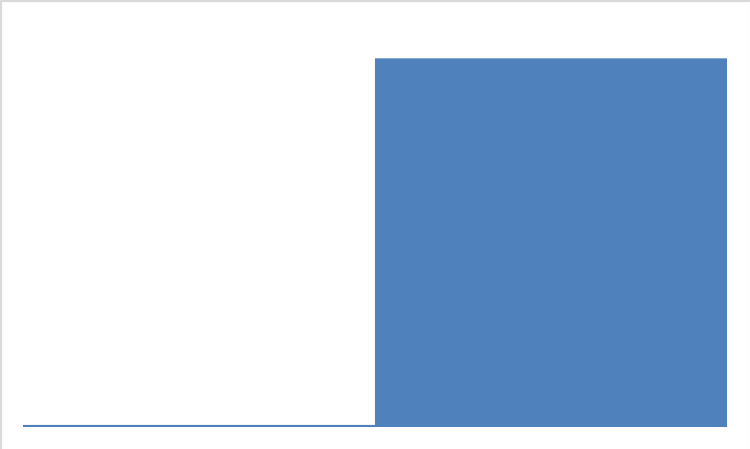
\includegraphics[width=0.2\textwidth, height=10mm]{methodology/images/mut17q21}\\
\textbf{loss 17} & 3 &  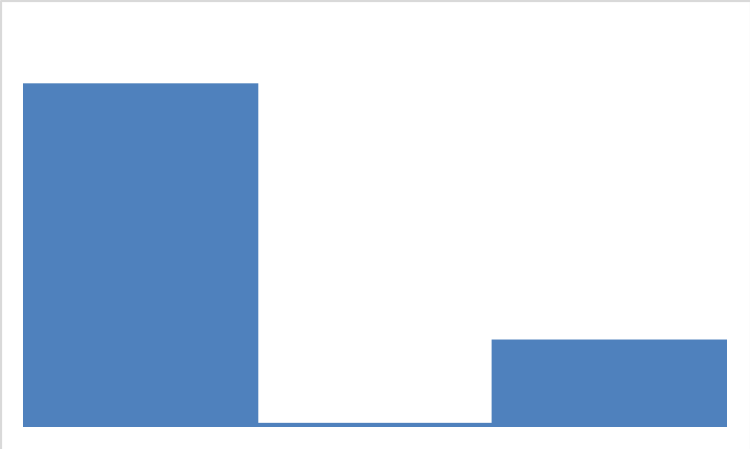
\includegraphics[width=0.2\textwidth, height=10mm]{methodology/images/loss_17}\\
\textbf{eta arrotondata} & 74 &  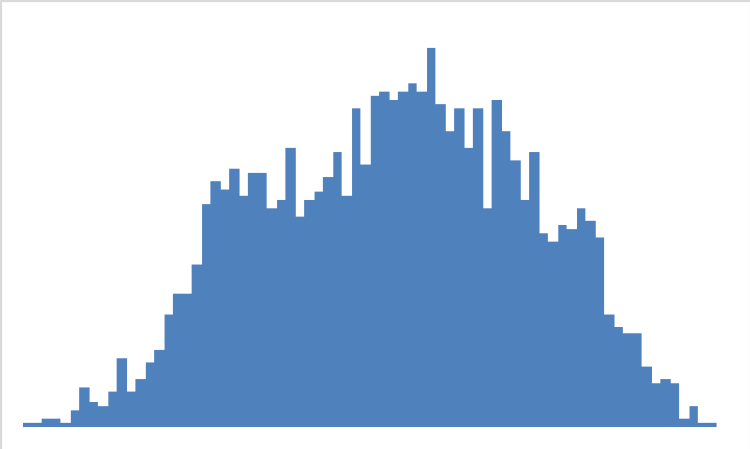
\includegraphics[width=0.2\textwidth, height=10mm]{methodology/images/eta_arrotondata}\\
\textbf{lateralit\`a} & 3 & 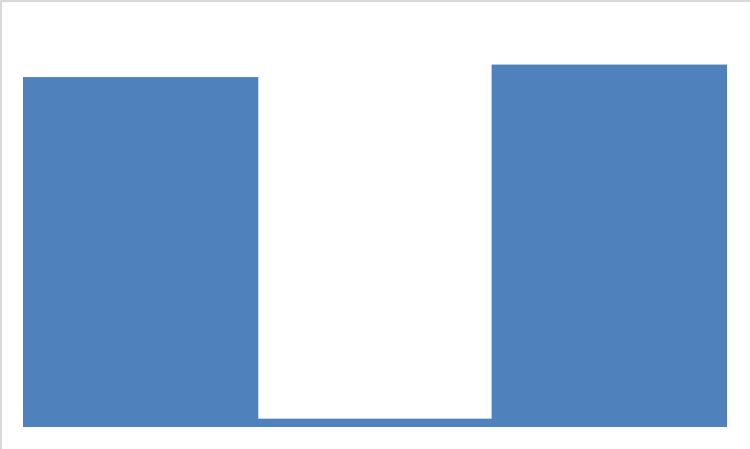
\includegraphics[width=0.2\textwidth, height=10mm]{methodology/images/lateralita} \\
\textbf{situ} & 5 & 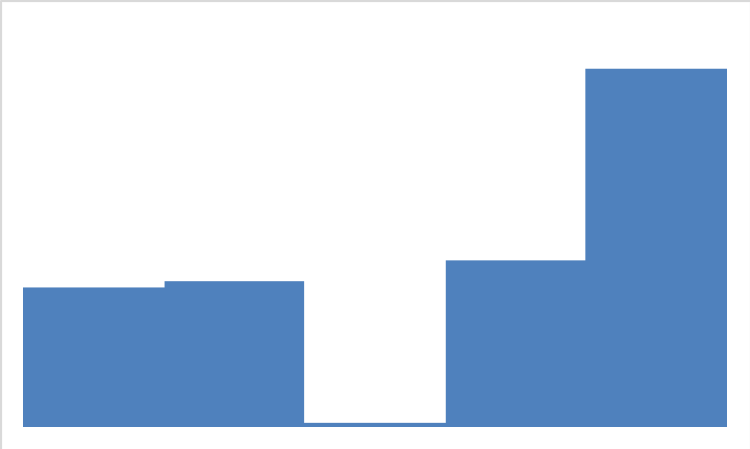
\includegraphics[width=0.2\textwidth, height=10mm]{methodology/images/situ} \\
\textbf{morfologia} & 5 & 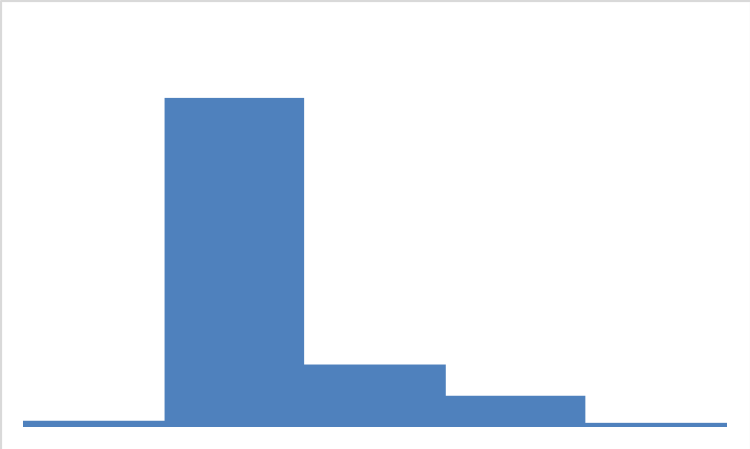
\includegraphics[width=0.2\textwidth, height=10mm]{methodology/images/morfologia} \\
\textbf{pT} & 23 & 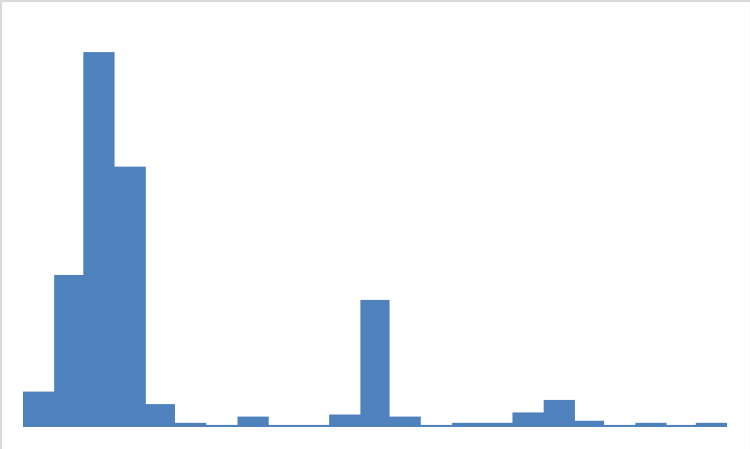
\includegraphics[width=0.2\textwidth, height=10mm]{methodology/images/pt} \\
\textbf{pN} & 6 & 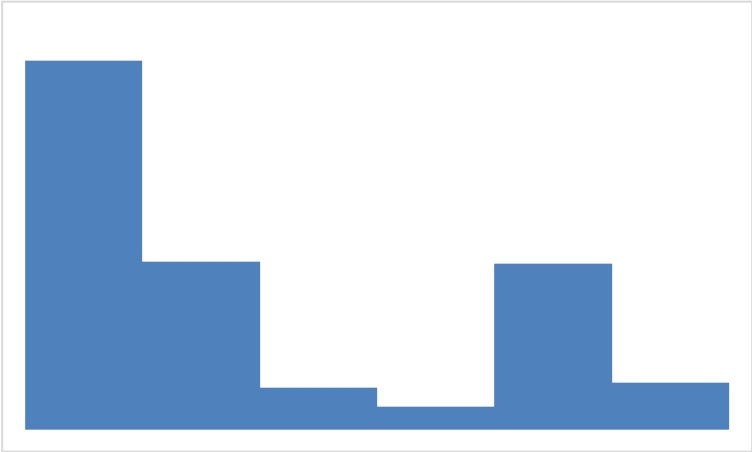
\includegraphics[width=0.2\textwidth, height=10mm]{methodology/images/pn} \\
\textbf{M} & 3 & 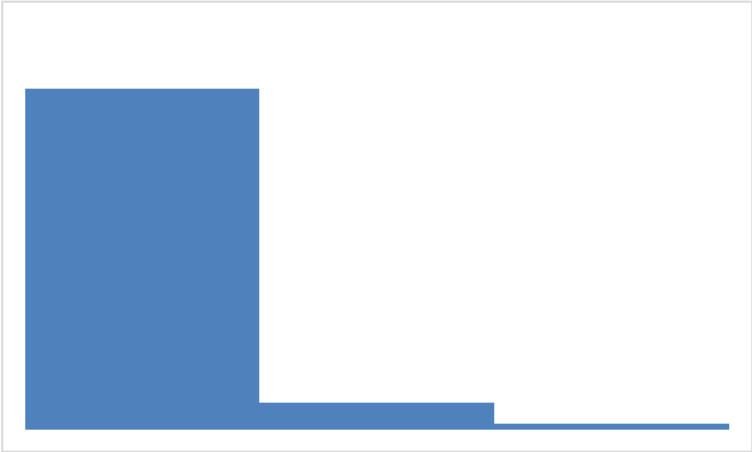
\includegraphics[width=0.2\textwidth, height=10mm]{methodology/images/m} \\
\textbf{differenziazione} & 5 & 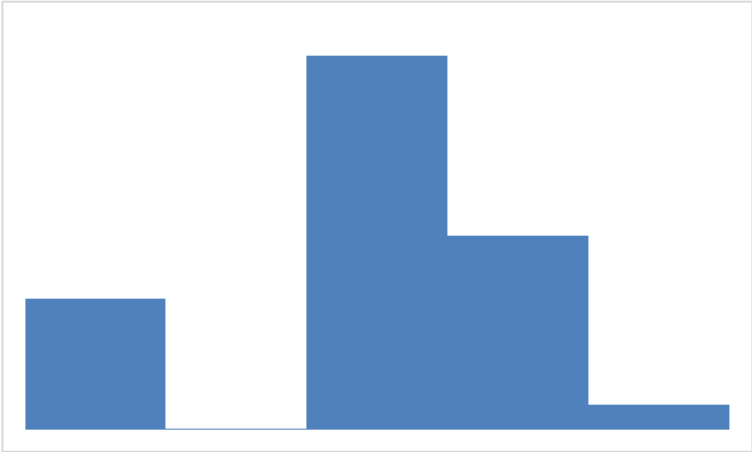
\includegraphics[width=0.2\textwidth, height=10mm]{methodology/images/differenziazione}  \\
\textbf{recettori estrogeni} & 40 & 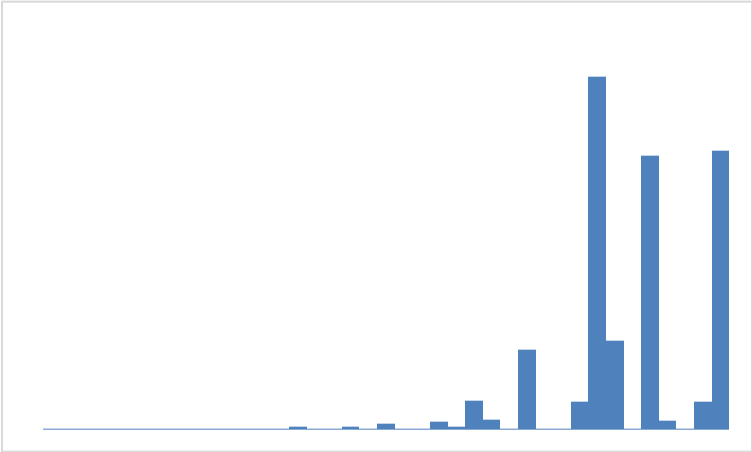
\includegraphics[width=0.2\textwidth, height=10mm]{methodology/images/recettori_estrogeni} \\
\textbf{recettori progestinici} & 40 & 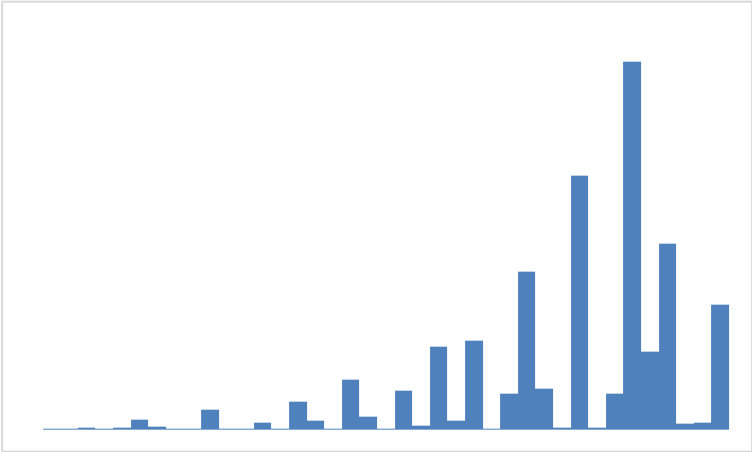
\includegraphics[width=0.2\textwidth, height=10mm]{methodology/images/recettori_progestinici}\\
\textbf{c erbB 2} & 4 & 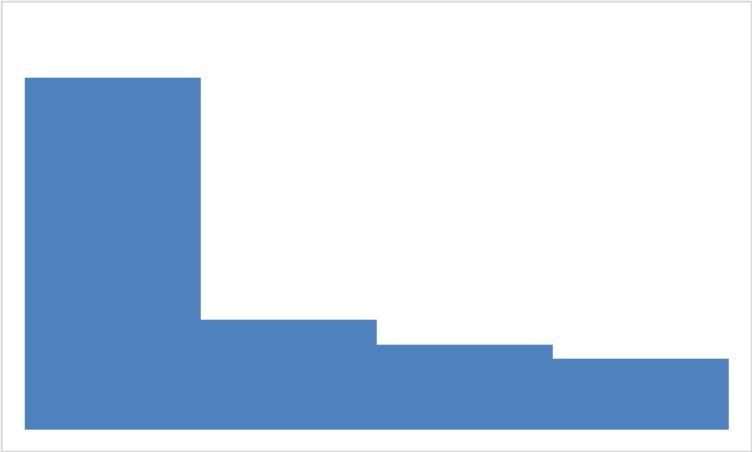
\includegraphics[width=0.2\textwidth, height=10mm]{methodology/images/c_erb_2}\\
\textbf{Ki67} & 52 & 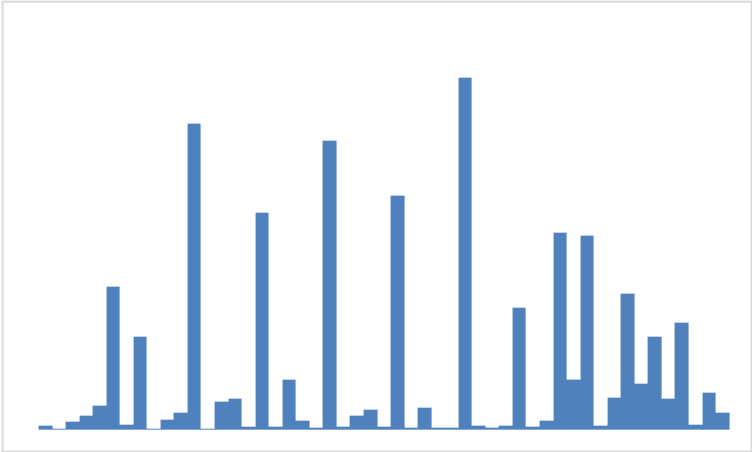
\includegraphics[width=0.2\textwidth, height=10mm]{methodology/images/ki67}\\
\textbf{FISHRation} & 5 &  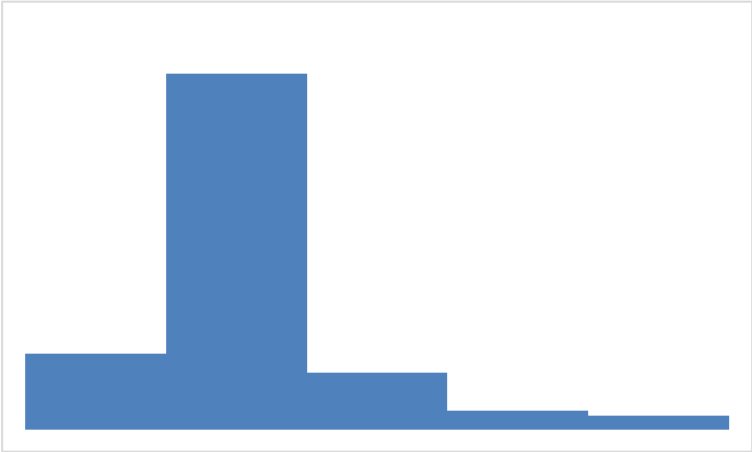
\includegraphics[width=0.2\textwidth, height=10mm]{methodology/images/fish}\\
\bottomrule
\end{tabularx}
\label{tab:datasetdistribution}
\end{table*}

\begin{table*}[htbp]
\centering
\caption{Data set preprocessing steps}
\begin{tabularx}{\textwidth}{@{} l Y @{}}
\toprule 
\textbf{Variable} & Action \\
\midrule 
\textbf{Codice globale} & Remove variable \\
\textbf{mut17q21} & Remove variable \\
\textbf{loss 17} & Remove variable \\
\textbf{eta arrotondata} & Bin into \enquote{$< 40$}, \enquote{$40-50$}, \enquote{$\geq 50$} \\
\textbf{lateralita} & Remove blanks and \enquote{sconosciuta} \\
\textbf{situ} & Remove blanks \\ \addlinespace
\textbf{morfologia} & Remove blanks and \enquote{unuseful} if performance on classification is subpar \\ \addlinespace
\textbf{pT} & Remove blanks and \enquote{unuseful}  \\
\textbf{pN} & Remove blanks and bin into \enquote{0} and \enquote{$\neq0$}\\
\textbf{M} & Remove blanks \\ 
\textbf{differenziazione} & Remove blanks and \enquote{Sconosciuto o non applicabile} \\ \addlinespace
\textbf{recettori estrogeni} & Remove blanks and bin into \enquote{negativo} if $\leq 10$,
		\enquote{debolmente positivo} if $\leq 50$, 
		\enquote{fortemente positivo} if $> 50$ \\ \addlinespace
\textbf{recettori progestinici} & Remove blanks and bin into \enquote{negativo} if $\leq 10$, 
		\enquote{debolmente positivo} if $\leq 50$, 
		\enquote{fortemente positivo} if $> 50$ \\ \addlinespace
\textbf{c erbB 2} & Remove blanks \\ 
\textbf{ki67} & Remove blanks and bin into \enquote{<14}, 
		\enquote{14-20}, \enquote{20-30}, \enquote{>30} \\ 
\textbf{FISH} & Remove variable \\
\bottomrule
\end{tabularx}
\label{tab:datasetpreprocess}
\end{table*}


\section{Validation Methodology} \label{sec:validation}
Having direct access to expert pathologists has not only helped in guiding research into the theoretical explainability properties of the system but also enabled their \textit{application-grounded evaluation} (see Section \ref{sec:evaluation-of-explainability}).
There are two main validation points of view to be addressed: the clinical (Subsection \ref{subsec:clinical-validation-methodology}) and the explainability (Subsection \ref{subsec:explainability-validation}), with the results of the latter depending on part on those of the former.
 
\subsection{Clinical Validation} \label{subsec:clinical-validation-methodology}
A validation of the methods carried out in this thesis in their adherence to established clinical literature is of paramount importance.
A failure on the Bayesian network's part in capturing the true relationships between the variables would hamper it in being able to give any meaningful representation of them.
For the experts to even start to trust the system or to be able to make sense of its outputs, it is vital that there be as little cognitive dissonance between their basic beliefs and expectations and those that they see represented in the system.

For this reason, the initial validation phase with the ICP concentrated on the clinical aspect.
The methodology chosen to clinically validate the system was for the ICP to formulate a series of natural language queries; each one of these questions was annotated with the queried variable and its value, together with the values of any evidence variables.
The experts included the expected reply to the queries together with its likelihood, based on the latest medical literature and their personal, knowledge-based expertise.
These questions can be abstracted as:
\begin{center}
\enquote{Given that the value of $var_1$ is $a_1$ and $\ldots$ and the value of $var_n$ is $a_n$, what is the probability that $var_{n+1}$ takes value $a_{n+1}$?}.	
\end{center}

The natural language questions formulated by the ICP can be classified along two axes:
\begin{itemize}
  \item based on their intended purpose: \textit{validation} vs. \textit{research}.
  The former questions' replies are known from established clinical literature and are the queries that will actually be used to validate the system from a clinical point of view.
  The latter are queries that don't have a definite clinical answer but that are nonetheless extremely interesting in helping to understand the types of questions a domain expert may want to ask the system.
  \item based on the way they may be answered: by a \textit{conditional probability query} (Definition \ref{def:conditional-probability}), a \textit{d-separation query} (Definition \ref{def:d-separation}) or an \textit{MPE query} (Definition \ref{def:mpe}).
\end{itemize}
The complete series of thirty questions has been organised according to the second criterion.
Appendixes \ref{app:conditionalprobability1} and \ref{app:conditionalprobability2} present fourteen questions that can be answered by conditional probability queries.
Appendix \ref{app:dseparation} shows a series of eight natural language questions that can be answered by running a d-separation query.
Appendix \ref{app:conditionalanddseparation} presents five questions that could be answered by a conditional probability query but also, at a higher level, by a d-separation query.
This is because what is being asked, is basically wether changing the value of the evidence variable has an influence on that of the target variable.
This could be answered by running multiple conditional probability queries and comparing the resulting target variable values or, more simply, by checking if the target and evidence variables are d-connected or not.
The first method would give a finer grained answer as it would also \textit{quantify} the magnitude of the effect of one variable on the other; checking for d-separation would only give a \textit{qualitative} answer, which may nonetheless be sufficient. 
Finally, Appendix \ref{app:mpe} shows three questions that are naturally mapped onto a query of the MPE type.

Most importantly at this stage, all questions can be implemented on the proof of concept system and consequently this shows a good coverage on the tool's part of the use cases that can be imagined by a domain expert.
If the system can, in principle, answer every question imagined by the expert then this is an indication that it conforms to her \textit{worldview} and thus could be well positioned to interact fruitfully with her.

The questions marked as \textit{validation} will be posed to the system, in autonomy, by the ICP's representatives, who will then compare the outputs with the result they would have expected, based on established medical literature and their expertise.
The columns containing the experts' expected results and their comments have been omitted from the natural language questions shown in Appendix \ref{app:natural-language-questions} and included directly in the discussion of the results in Subsection \ref{subsec:clinical-validation-results}, alongside the system's outputs.
If the system's outputs conform to the experts' preconceived ideas in a high number of cases (as confirmed by the experts themselves) then the system can be said to have been \textit{clinically validated}.
This is important because the enabling condition for the user to trust the predictions made by the software is that these shouldn't be in strong discordance with her existing beliefs.
Not having a strong \textit{cognitive dissonance} is a \textit{necessary} - but not sufficient - condition to enable trust and therefore explainability.

\subsection{Explainability Validation} \label{subsec:explainability-validation}
In general, there is strong resistance to novelty in the field of medicine, both for ethical reasons and because of the need for clinicians to be conservative in attending to established best practices in the field.
Any tool that is too onerous in terms of time and cognitive load is liable to remain underutilised.
In this field, \textit{a tool must therefore only be the means by which a question is answered}, not itself become a question; the methods developed in this thesis aim to conform to this objective, barring the experimental nature of the software and the consequent lack of refinement of its interface.
The need for a comprehensible and efficient tool is especially present because the goal of a pathologist is to arrive at a diagnosis, containing the elements useful to define prognosis and therapeutical approach, in the briefest time possible.
The main reasons are ethical, since for a patient waiting for a report is extenuating, and clinical, because a timely diagnosis is the first factor at the base of life expectancy.
Obviously, the highest possible accuracy is always strived for.
The clinical field and that of biomedicine are forced to embrace uncertainty, as this is an integral part of their practice.
Consequently, any tool able to support in comprehension and decision-making is automatically useful, once it has been clinically validated; in other words, even though a specific system may not be decisive or applicable to all reviewed cases, it will nonetheless be taken into account.

Thus, a system validated in terms of its adherence to clinical literature could then also meaningfully be validated from an explainability point of view.
The main question to be addressed is its capacity to relate to the expert user.
Is the system able to engender the user's trust?
In doing so, is she able to extract more knowledge from existing data when using the system than not?
Especially in cases where there may be a dearth of data, can the expert maximise the benefit from the available information?
Does the user subjectively feel that the system may positively impact her work?
These are all hard questions to answer, as there is a very high degree of subjectivity involved.
Thus to attempt to answer them, the chosen methods were borrowed from the social sciences.

In an earlier stage, the experts were introduced to the system in prototype form and instructed on the use cases it offered.
This process would enable the collection of feedback on the functionalities of the system and help in shaping its subsequent design.

The finalised system was, in a later phase (early August 2019), provided to the experts at the ICP for use in their daily work.
To quantify the performance of the system, as perceived by its users in a real setting over an extended period of time, a follow-up was done after three weeks by way of an \enquote{explainability evaluation questionnaire}, designed to test the gaps identified in Chapter \ref{chap:literature-review}.
The full questionnaire can be found in Appendix \ref{app:questionnaire}.

The \enquote{explainability evaluation questionnaire} presents five sections:
\begin{itemize}
  \item \textit{confidence}: aimed at assessing wether the use of the system incremented the confidence the clinician felt in making her decisions;
  \item \textit{features}: to understand in more detail which interaction modes were perceived as most useful and the subjective reasons for this.
  Of particular interest is the understanding of the perceived quality of the dialogical interaction modes and of the \enquote{pseudo-MPE} query;
  \item \textit{time}: questions focusing on the the temporal element, mainly the time needed to understand various explanations offered by the system.
  This element is often overlooked in the relevant xAI literature (see Section \ref{sec:explainability-in-bayesian-networks});
  \item \textit{tool}: general questions regarding the use of tool and if any important use-case was felt to be missing;
  \item \textit{clinical}: investigating if the tool was clinically relevant in day-to-day work.
  Unlike the clinical validation presented in Subsection \ref{subsec:clinical-validation-methodology}, these questions investigate \textit{a posteriori} the use of the tool and as such should provide a broader evaluation of its clinical relevance;
  \item \textit{satisfaction}: simple question asking to rate the general satisfaction with the proof of concept system.
\end{itemize}

As discussed throughout Chapter \ref{chap:literature-review} and summarised in Section \ref{sec:literature-review-summary}, one of the main gaps in the field of explainable AI is the absence of real-world validation of the - supposedly - explainable models.
The objective of the questionnaire is to act as an \textit{application-grounded evaluation}, in the taxonomy proposed by \citet{doshi2017towards} and presented in Section \ref{sec:evaluation-of-explainability}, and thus provide what is considered the gold standard for the evaluation of a machine learning system.
Also included, since it is almost always neglected in literature, is a focus on the \textit{temporal element} of the explanations that was noted as important by \citet{gilpin2018explaining}.
Of particular interest is evaluating the Bayesian network - underlying the tool's capabilities - in its capacity to surface cogent explanations for the target user; the questionnaire inflects the questions in order to identify which particular characteristics of the system and BN were perceived by the user as the most useful in order to gain an understanding of the underlying data set.
As noted in Section \ref{sec:explainability-in-bayesian-networks}, by acknowledging the psychological characteristics of an explanation identified by \citet{miller2018explanation}, explanations have various essential characteristics that seem to also be inherent in BNs; the questionnaire thus seeks to understand if these are actually present and perceived as useful, in the sense of enabling explainability, by the domain experts.

The questionnaire is not the only source of the results relating to the \textit{application-grounded evaluation} of the developed system; similarly to \citep{stumpf2009interacting} in their \enquote{think-aloud experiment}, many results and details throughout Chapter \ref{chap:results} will be the outcome of observing and listening to the expert users while they were engaging with the system.
We refer to these as \enquote{informal explainability evaluation results} contrasting them with the \enquote{formal explainability evaluation results} that will be the outcomes of the questionnaire.



%%%%
%%%% RESULTS
%%%%

\chapter{Results}\label{chap:results}

%%%%
%%%% CONCLUSIONS
%%%%

\chapter{Conclusions}\label{chap:conclusions}

\section{Critique of MPE paper}

\chapter{Future developments}\label{chap:future-developments}



\appendix %optional, use only if you have an appendix


\backmatter

\chapter{Glossary} %optional

%\bibliographystyle{alpha}
%\bibliographystyle{dcu}
\bibliographystyle{plainnat}
\bibliography{biblio}

%\cleardoublepage
%\theindex %optional, use only if you have an index, must use
	  %\makeindex in the preamble


\end{document}
